% Applied Acoustics submission — elsarticle, Elsevier review format
% (double-spaced single column with line numbers, as required for peer review)
\documentclass[review]{elsarticle}

\usepackage{amsmath,amssymb}
\usepackage{graphicx}
\usepackage{booktabs}
\usepackage{multirow}
\usepackage{xcolor}
\usepackage{lineno}
\usepackage{url}

\graphicspath{{figures/}}

%                       
% Multi-seed results of the proposed configuration (script 12,
% results/logmel_multiseed_results.txt). Filled from the 10-seed run.
%                       
\newcommand{\msFanAuc}{0.941}    \newcommand{\msFanAucSd}{0.009}    \newcommand{\msFanAucCI}{[0.934, 0.946]}
\newcommand{\msPumpAuc}{0.945}   \newcommand{\msPumpAucSd}{0.011}   \newcommand{\msPumpAucCI}{[0.938, 0.952]}
\newcommand{\msSliderAuc}{0.988} \newcommand{\msSliderAucSd}{0.006} \newcommand{\msSliderAucCI}{[0.985, 0.992]}
\newcommand{\msValveAuc}{0.962}  \newcommand{\msValveAucSd}{0.026}  \newcommand{\msValveAucCI}{[0.945, 0.976]}
\newcommand{\msFanPauc}{$0.809 \pm 0.027$}   \newcommand{\msPumpPauc}{$0.879 \pm 0.027$}
\newcommand{\msSliderPauc}{$0.970 \pm 0.007$}\newcommand{\msValvePauc}{$0.866 \pm 0.086$}
\newcommand{\msFanFone}{$0.758 \pm 0.045$}   \newcommand{\msPumpFone}{$0.696 \pm 0.091$}
\newcommand{\msSliderFone}{$0.911 \pm 0.045$}\newcommand{\msValveFone}{$0.681 \pm 0.123$}
\newcommand{\msFanFcal}{$0.791 \pm 0.020$}   \newcommand{\msPumpFcal}{$0.760 \pm 0.041$}
\newcommand{\msSliderFcal}{$0.925 \pm 0.011$}\newcommand{\msValveFcal}{$0.731 \pm 0.107$}

\journal{Applied Acoustics}

% Insert the graphical abstract inline, right after the author/affiliation
% block and before the text abstract, on the same title page (rather than
% eslarticle's default behaviour of a separate page that re-prints the
% title/authors). \pprintMaketitle is copied verbatim from elsarticle.cls
% with one added line: \unvbox\mygrabsbox before the first \hrule.
\makeatletter
\newbox\mygrabsbox
\newenvironment{mygraphicalabstract}{%
  \global\setbox\mygrabsbox=\vbox\bgroup
  \hsize=\textwidth\def\baselinestretch{1}%
  \noindent\unskip{\Large Graphical Abstract}\par\vskip8pt\noindent\ignorespaces}
  {\egroup}

\def\pprintMaketitle{\clearpage
  \iflongmktitle\if@twocolumn\let\columnwidth=\textwidth\fi\fi
  \resetTitleCounters
  \def\baselinestretch{1}%
  \printFirstPageNotes
  \begin{\elsarticletitlealign}%
 \thispagestyle{pprintTitle}%
   \def\baselinestretch{1}%
    \Large\@title\par\vskip18pt%
    \ifx\@elsarticlenewpageafter\newpage@after@title%
      \newpage
    \fi%
    \ifdoubleblind
      \vspace*{2pc}
    \else
      \normalsize\elsauthors\par\vskip10pt
      \footnotesize\itshape\elsaddress\par\vskip36pt
    \fi
    \ifx\@elsarticlenewpageafter\newpage@after@author%
      \newpage
    \fi%
    \ifvoid\mygrabsbox\else\unvbox\mygrabsbox\par\vskip10pt\fi
    \hrule\vskip12pt
    \ifvoid\absbox\else\unvbox\absbox\par\vskip10pt\fi
    \ifvoid\keybox\else\unvbox\keybox\par\vskip10pt\fi
    \hrule\vskip12pt
    \ifx\@elsarticlenewpageafter\newpage@after@abstract%
      \newpage
    \fi%
    \end{\elsarticletitlealign}%
    \gdef\thefootnote{\arabic{footnote}}%
  }
\makeatother

\begin{document}
\linenumbers

\begin{frontmatter}

\title{Lightweight CPU-bound convolutional neural networks for acoustic anomaly detection of industrial machinery under severe noise: spectral representation, class imbalance, and hardware-decoupled deployment}

\author[HAU]{Sakar Mohammad Raziul Hasan Rifat}
\author[HAU]{Akter Labani}
\author[HAU]{Tao Zhang\corref{cor1}}
\ead{taozhang2021@hau.edu.cn}
\author[HAU]{Saleh Mahamat Aboubakar OUSMANE}
\author[HAU]{Boudjelkha Mohammed Djamel EDDINE}

\cortext[cor1]{Corresponding author.}
\affiliation[HAU]{organization={Department of Mechanical Engineering, Huai'an University},
            city={Huai'an},
            state={Jiangsu},
            country={China}}

\begin{mygraphicalabstract}
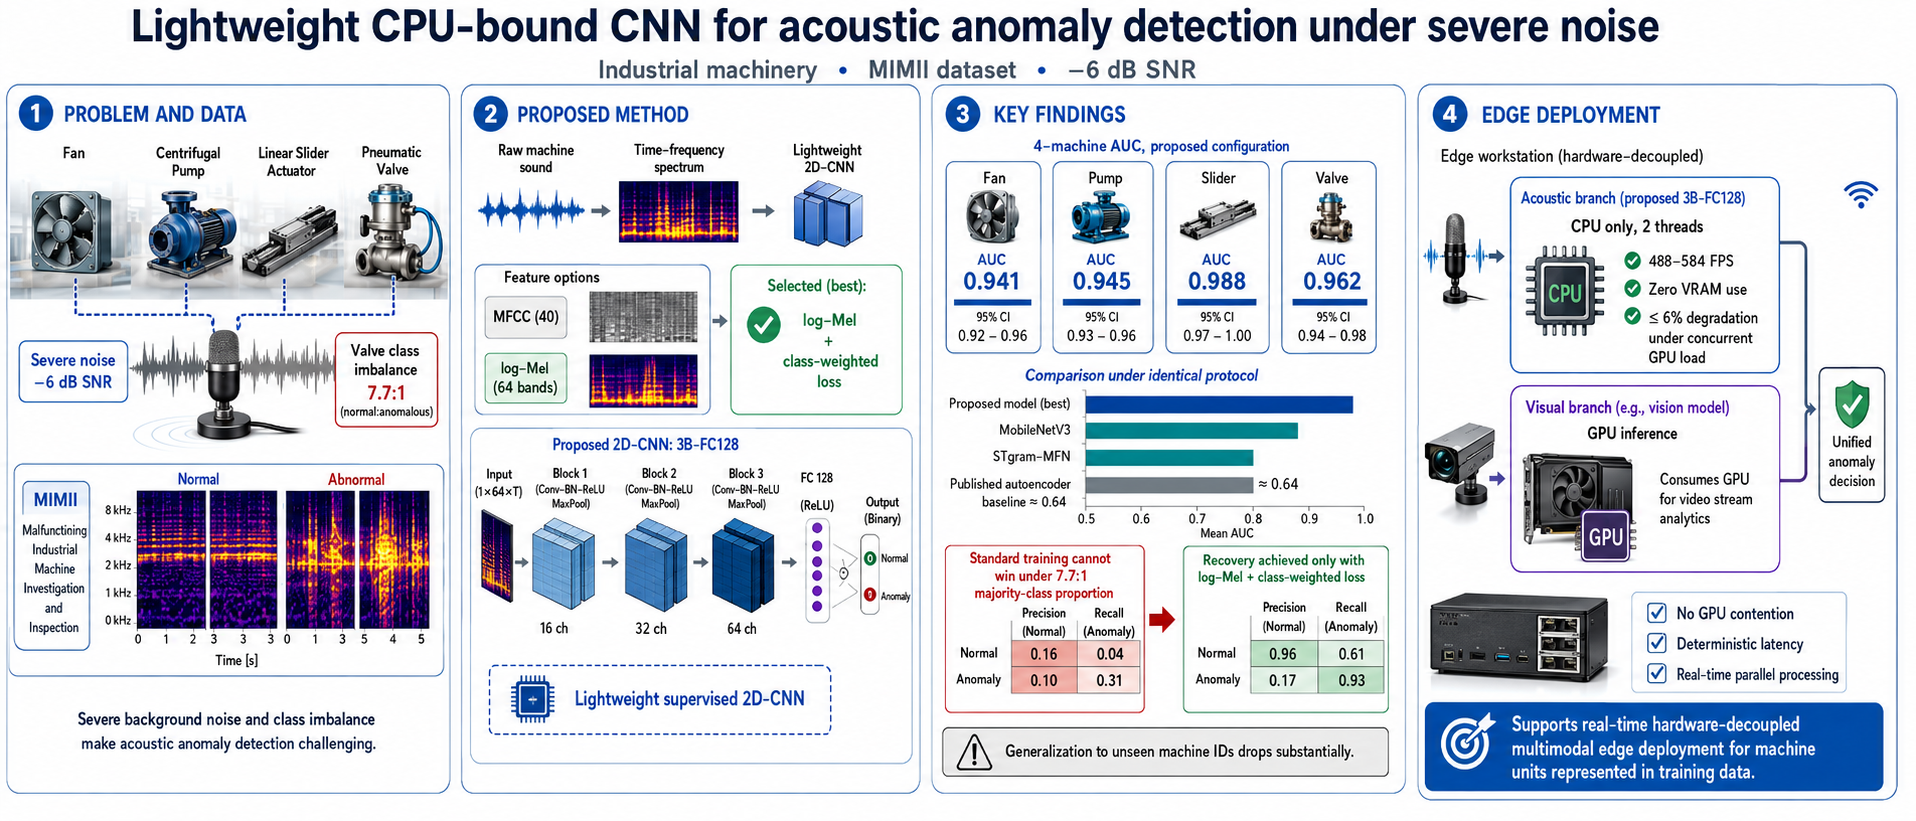
\includegraphics[
  width=\textwidth,
  height=0.32\textheight,
  keepaspectratio
]{graphical_abstract.png}
\end{mygraphicalabstract}

\begin{abstract}
Acoustic condition monitoring of industrial machinery must contend with severe background noise, class imbalance, and edge hardware shared with concurrent visual workloads. This paper presents a systematic study of a lightweight two-dimensional convolutional neural network (3B-FC128) for supervised acoustic anomaly detection on the MIMII dataset at $-6$\,dB. Across ten seeds, the proposed log-Mel, class-weighted configuration attains mean AUC--ROC of \msFanAuc{} (fan), \msPumpAuc{} (pump), \msSliderAuc{} (slider), and \msValveAuc{} (valve), above the published autoencoder baseline ($\approx 0.64$) and our own autoencoder reproduction. Under one identical protocol it also attains the best mean AUC of three compared supervised architectures, ahead of MobileNetV3 and a heavier STgram-MFN fusion network, and never collapses to chance on any seed, unlike the fusion baseline. The 7.7:1 imbalanced valve category collapses to majority-class prediction under standard training; recovery requires jointly applying log-Mel input and class-weighted loss, since MFCC features remain collapsed even when re-weighted and single-run valve results are seed-unstable, motivating multi-seed evaluation. Ablations over six architecture variants, two spectral representations, three SNR levels, and leave-one-machine-out cross-validation characterize capacity, representation, noise, and generalization effects. Finally, the lighter MFCC variant of the proposed model sustains 488--584 frames per second at two CPU threads with zero VRAM use and at most 6\% degradation under concurrent GPU load; the log-Mel variant is $\sim$2$\times$ costlier per inference but still clears the real-time requirement by orders of magnitude, supporting hardware-decoupled multimodal deployment at the industrial edge for units represented in training data.
\end{abstract}

\begin{keyword}
acoustic anomaly detection \sep machine condition monitoring \sep convolutional neural network \sep MIMII \sep class imbalance \sep edge computing
\end{keyword}

\end{frontmatter}

% ==================================================================
\section{Introduction}
\label{sec:intro}

The integrity of rotating and reciprocating industrial machinery---ventilation fans, centrifugal pumps, linear slide actuators, and pneumatic valves---is critical to operational continuity in manufacturing, energy, and process industries. Acoustic condition monitoring offers a non-invasive, low-cost diagnostic modality, since anomalous mechanical states (bearing wear, seal degradation, leakage, rail contamination) manifest as characteristic deviations of the radiated acoustic spectrum before functional failure~\cite{purohit2019mimii,koizumi2019toyadmos}. Real industrial environments, however, routinely exhibit background noise at or above the level of the monitored source, producing an adverse signal-to-noise regime that severely challenges feature discrimination.

The MIMII dataset~\cite{purohit2019mimii} provides standardized recordings of four machine types under controlled SNR conditions ($-6$, $0$, and $+6$\,dB) and has become, together with the DCASE Challenge Task~2 series~\cite{koizumi2020dcase,kawaguchi2021dcase,dohi2022dcase}, the de facto benchmark for anomalous sound detection (ASD) of machinery. At the $-6$\,dB operating point, the autoencoder baseline of Purohit et al.~\cite{purohit2019mimii} achieves an average area under the ROC curve (AUC) of only about $0.64$, indicating that reconstruction-based unsupervised detection degrades strongly under severe noise. When labelled abnormal recordings are available---as is increasingly the case in plants that log confirmed failure events---a discriminative supervised classifier can instead learn the decision boundary directly, a strategy explored by DCASE participants with competitive results~\cite{giri2020selfsupervised,liu2022stgram}.

Two further obstacles arise in practice. First, anomalous machine states are rare by design, so training data are strongly imbalanced (up to 8.2:1 normal-to-abnormal in MIMII), which biases standard losses toward trivial all-normal solutions. Second, the computing node at the industrial edge is typically shared: visual inspection models occupy most or all of the GPU memory budget, so an acoustic model that also demands GPU residency creates contention. Running acoustic inference exclusively on the CPU eliminates video-memory contention entirely, provided CPU throughput and latency satisfy the application's monitoring rate.

This paper presents a systematic experimental study of a deliberately lightweight two-dimensional convolutional neural network (2D-CNN), designated 3B-FC128, for supervised acoustic anomaly detection on MIMII at $-6$\,dB. The novelty lies not in the architecture---compact CNNs and transformers for machinery ASD are by now well established~\cite{liu2022stgram,zhang2026tinyast}---but in characterizing, with statistical rigor, how such a model behaves under three under-examined and practically decisive stresses: extreme class imbalance, single-run seed instability, and shared CPU/GPU edge hardware. The contributions are:

\begin{enumerate}
\item \textbf{Multi-seed statistical evaluation under extreme noise.} The proposed log-Mel + class-weighted configuration is evaluated over ten random seeds with bootstrap confidence intervals, partial AUC (pAUC, $\mathrm{FPR}\le 0.1$), and calibrated decision thresholds, demonstrating that a 2--3.3\,M-parameter discriminative model substantially outperforms autoencoder baselines at $-6$\,dB.
\item \textbf{Characterization of class-imbalance-induced decision collapse and its remedy.} The valve category (7.7:1 imbalance) collapses to majority-class prediction under standard training. We show that recovery requires the \emph{joint} use of log-Mel spectrogram input and class-weighted loss---re-weighting alone leaves MFCC features collapsed---and we quantify the seed instability of single-run valve results, which has not been reported in prior MIMII studies.
\item \textbf{Representation and capacity ablations.} Controlled comparisons of MFCC (40 coefficients) versus log-Mel (64 bands) input, and of six CNN variants spanning two to four convolutional blocks and 64--256-unit classifiers, identify the three-block, 128-unit configuration as the best accuracy--latency operating point.
\item \textbf{Honest generalization analysis.} Leave-one-machine-ID-out cross-validation quantifies the (substantial) performance drop when the model must generalize to unseen machine units, delimiting the operating envelope of the supervised approach.
\item \textbf{Fair multi-seed baseline comparison.} Under one identical protocol, the proposed model attains the best mean AUC of the three supervised architectures compared---ahead of a lightweight MobileNetV3 on every machine and a heavier STgram-MFN spectral--temporal fusion baseline on average---and never collapses to chance on any of forty seed-runs, unlike the fusion baseline, while remaining half the size and roughly twice the CPU throughput of the latter.
\item \textbf{Hardware-decoupled deployment benchmark.} Thread-count sweeps, latency distributions, and CPU-versus-GPU comparisons on a six-core AMD Ryzen 5 7500F with a co-resident NVIDIA RTX 5070 under full visual load show 488--584 frames per second (FPS) of acoustic throughput for the MFCC variant of the proposed model at two threads with zero VRAM use and at most 6\% interference degradation.
\end{enumerate}

The remainder of the paper is organized as follows. Section~\ref{sec:related} reviews related work. Section~\ref{sec:methods} describes the dataset, feature pipelines, architecture, training, and evaluation protocols. Section~\ref{sec:results} presents detection results, including the collapse analysis and multi-seed validation. Section~\ref{sec:ablation} reports ablations, SNR robustness, baseline comparisons, and machine-ID generalization. Section~\ref{sec:deploy} analyses deployment. Sections~\ref{sec:discussion}--\ref{sec:conclusion} discuss findings, limitations, and conclusions.

% ==================================================================
\section{Related work}
\label{sec:related}

\subsection{Anomalous sound detection for industrial machinery}
The MIMII dataset~\cite{purohit2019mimii} established machinery ASD as a benchmark task; the DCASE Challenge Task~2 series~\cite{koizumi2020dcase,kawaguchi2021dcase,dohi2022dcase} extended it with domain shift across machine identifiers and operating conditions (MIMII~DUE~\cite{tanabe2021mimiidue}). Early systems were predominantly unsupervised and reconstruction-based: autoencoders trained on normal data flag samples with large reconstruction error~\cite{purohit2019mimii,koizumi2019toyadmos}, with refinements such as interpolation DNNs~\cite{suefusa2020idnn}. Reconstruction approaches degrade in low-SNR regimes because the error is dominated by the noise floor rather than machine-state-dependent components. Density and one-class alternatives, e.g.\ variational autoencoders~\cite{kingma2014vae} and deep support vector data description~\cite{ruff2018deepsvdd}, share the assumption that a compact model of normality is learnable, which likewise erodes under severe additive noise.

A second line of work converts ASD into a discriminative task. Self-supervised classification over machine identifiers~\cite{giri2020selfsupervised}, spectral--temporal fusion classifiers (STgram-MFN)~\cite{liu2022stgram}, ArcFace-margin classifiers with Gaussian-mixture scoring~\cite{wu2023arcface}, and transfer learning from image backbones~\cite{muller2021transfer} consistently outperform reconstruction baselines when (pseudo-)labels are available. This momentum has continued in recent work: generative-adversarial models such as MaSGAN attack the scarcity of abnormal samples directly~\cite{yin2025masgan}, while compact supervised transformers report strong noise robustness on MIMII while remaining small enough for edge use~\cite{zhang2026tinyast}, confirming both the value of supervision under severe noise and the field's shift toward lightweight, deployable models. The present work adopts fully supervised binary classification, exploiting MIMII's labelled abnormal recordings; the protocol implications relative to unsupervised DCASE systems are made explicit in Section~\ref{sec:baselines}.

\subsection{CNNs on time--frequency representations}
Treating audio as a two-dimensional time--frequency image processed by 2D-CNNs is well established for environmental sound classification~\cite{piczak2015esc,salamon2017deep}. For embedded audio, compact CNNs for keyword spotting~\cite{zhang2017helloedge} and mobile-efficient designs~\cite{howard2017mobilenets} demonstrate that small, carefully sized networks retain competitive accuracy at a fraction of the inference cost. Transformer-based audio models such as AST~\cite{gong2021ast} and large pretrained audio networks~\cite{kong2020panns} achieve state-of-the-art accuracy on general audio benchmarks but carry parameter counts (87\,M+) and latency that are impractical for CPU-only industrial edge nodes, which motivates the lightweight CNN class studied here. The choice of time--frequency representation is itself an open question: beyond the log-Mel and MFCC inputs compared here, recent studies argue that psychoacoustically motivated or learned front-ends can be more discriminative for machinery fault detection~\cite{wissbrock2024more,liu2022stgram}, a point we revisit when scoping our representation claim (Sections~\ref{sec:representation} and~\ref{sec:limitations}). Recent lightweight transformer variants narrow this gap---e.g.\ a reduced Audio Spectrogram Transformer ($\approx$1\,M parameters) attains competitive robustness on the MIMII pump subset across SNR levels~\cite{zhang2026tinyast}---confirming that compact attention-based and convolutional models are now the practical design point for machinery ASD. Such models are nonetheless evaluated in isolation on dedicated hardware; to our knowledge none characterize operation on CPU while a co-resident GPU is saturated by a concurrent visual workload, which is precisely the deployment regime examined in Section~\ref{sec:deploy}.

\subsection{Class imbalance}
Class imbalance is endemic to fault detection. Data-level remedies (e.g.\ SMOTE~\cite{chawla2002smote}) synthesize minority samples, while loss-level remedies re-weight or re-focus the objective (class-weighted cross-entropy; focal loss~\cite{lin2017focal}). For fixed audio datasets, loss-level re-weighting through the positive-class weight of binary cross-entropy is attractive because it modifies neither the data distribution nor the inference path. This work shows, however, that re-weighting alone is insufficient under severe noise when the input representation discards the discriminative structure of the minority class (Section~\ref{sec:representation}).

\subsection{Edge deployment and resource partitioning}
Model compression---quantization~\cite{jacob2018quantization}, distillation~\cite{hinton2015distillation}---reduces the cost of a given network, and serving systems address multi-model scheduling~\cite{crankshaw2017clipper}. The complementary scenario studied here, in which a CPU-resident acoustic model coexists with a GPU-saturating visual workload on one commodity node, has received little systematic benchmarking in the ASD literature; Section~\ref{sec:deploy} provides controlled interference measurements for this case.

% ==================================================================
\section{Materials and methods}
\label{sec:methods}

\subsection{Dataset}
\label{sec:dataset}
All detection experiments use the MIMII dataset~\cite{purohit2019mimii} at the $-6$\,dB SNR partition (with $0$ and $+6$\,dB used in the SNR sweep of Section~\ref{sec:snr}). Recordings are 10-s single-channel WAV files at 16\,kHz from four machine types (fan, pump, slider, valve), each comprising four machine identifiers (id\_00, id\_02, id\_04, id\_06) and labelled normal or abnormal at file level. Table~\ref{tab:dataset} summarizes the composition. Anomalous conditions are machine-specific: rotor imbalance and contamination (fan), leakage and clogging (pump), rail contamination and lubrication failure (slider), and seal degradation and blockage (valve). One model instance is trained per machine type.

\begin{table}[t]
\centering
\caption{Composition of the MIMII $-6$\,dB partition used in this study.}
\label{tab:dataset}
\begin{tabular}{lcccc}
\toprule
Machine & Normal & Abnormal & Total & Imbalance \\
\midrule
Fan    & 4{,}075 & 1{,}475 & 5{,}550 & 2.8:1 \\
Pump   & 3{,}749 & 456     & 4{,}205 & 8.2:1 \\
Slider & 3{,}204 & 890     & 4{,}094 & 3.6:1 \\
Valve  & 3{,}691 & 479     & 4{,}170 & 7.7:1 \\
\bottomrule
\end{tabular}
\end{table}

Unless stated otherwise, experiments use a deterministic 80/20 train/test partition drawn with a fixed-seed generator; the test partition is never used for training. The single-seed comparisons of Sections~\ref{sec:representation} and~\ref{sec:arch} that motivate the proposed representation and architecture are exploratory analyses on this partition, not a held-out validation set; the confirmatory evidence for both choices is the ten-seed protocol of Section~\ref{sec:protocol}, which redraws the partition and the network initialization independently per seed and shares only one seed (42) with the exploratory analysis.

\subsection{Spectral representations}
\label{sec:features}
Two time--frequency representations are compared, both computed with librosa~\cite{mcfee2015librosa} (v0.11) at the native 16\,kHz rate, using librosa's default short-time parameters (2048-sample FFT, 512-sample hop, Hann window), and padded or truncated to 400 frames.

\paragraph{MFCC (40 coefficients)} Mel-frequency cepstral coefficients~\cite{davis1980mfcc} (\texttt{librosa.feature.mfcc}, \texttt{n\_mfcc=40}), giving an input tensor of shape $(1,40,400)$. The discrete cosine transform (DCT) step decorrelates the log-Mel filterbank energies, compacting the spectral envelope but discarding inter-band co-occurrence structure.

\paragraph{Log-Mel spectrogram (64 bands)} Mel filterbank energies (\texttt{librosa.feature.melspectrogram}, \texttt{n\_mels=64}) converted to decibels (\texttt{librosa.power\_to\_db}, \texttt{ref=np.max}) and standardized per sample (zero mean, unit variance), giving an input tensor of shape $(1,64,400)$. The full spectral energy distribution across bands is retained.

Figure~\ref{fig:spectrograms} shows exemplar normal and abnormal log-Mel spectrograms for the four machine types at $-6$\,dB; the broadband noise floor that dominates all panels illustrates the difficulty of the regime.

\begin{figure*}[t]
\centering
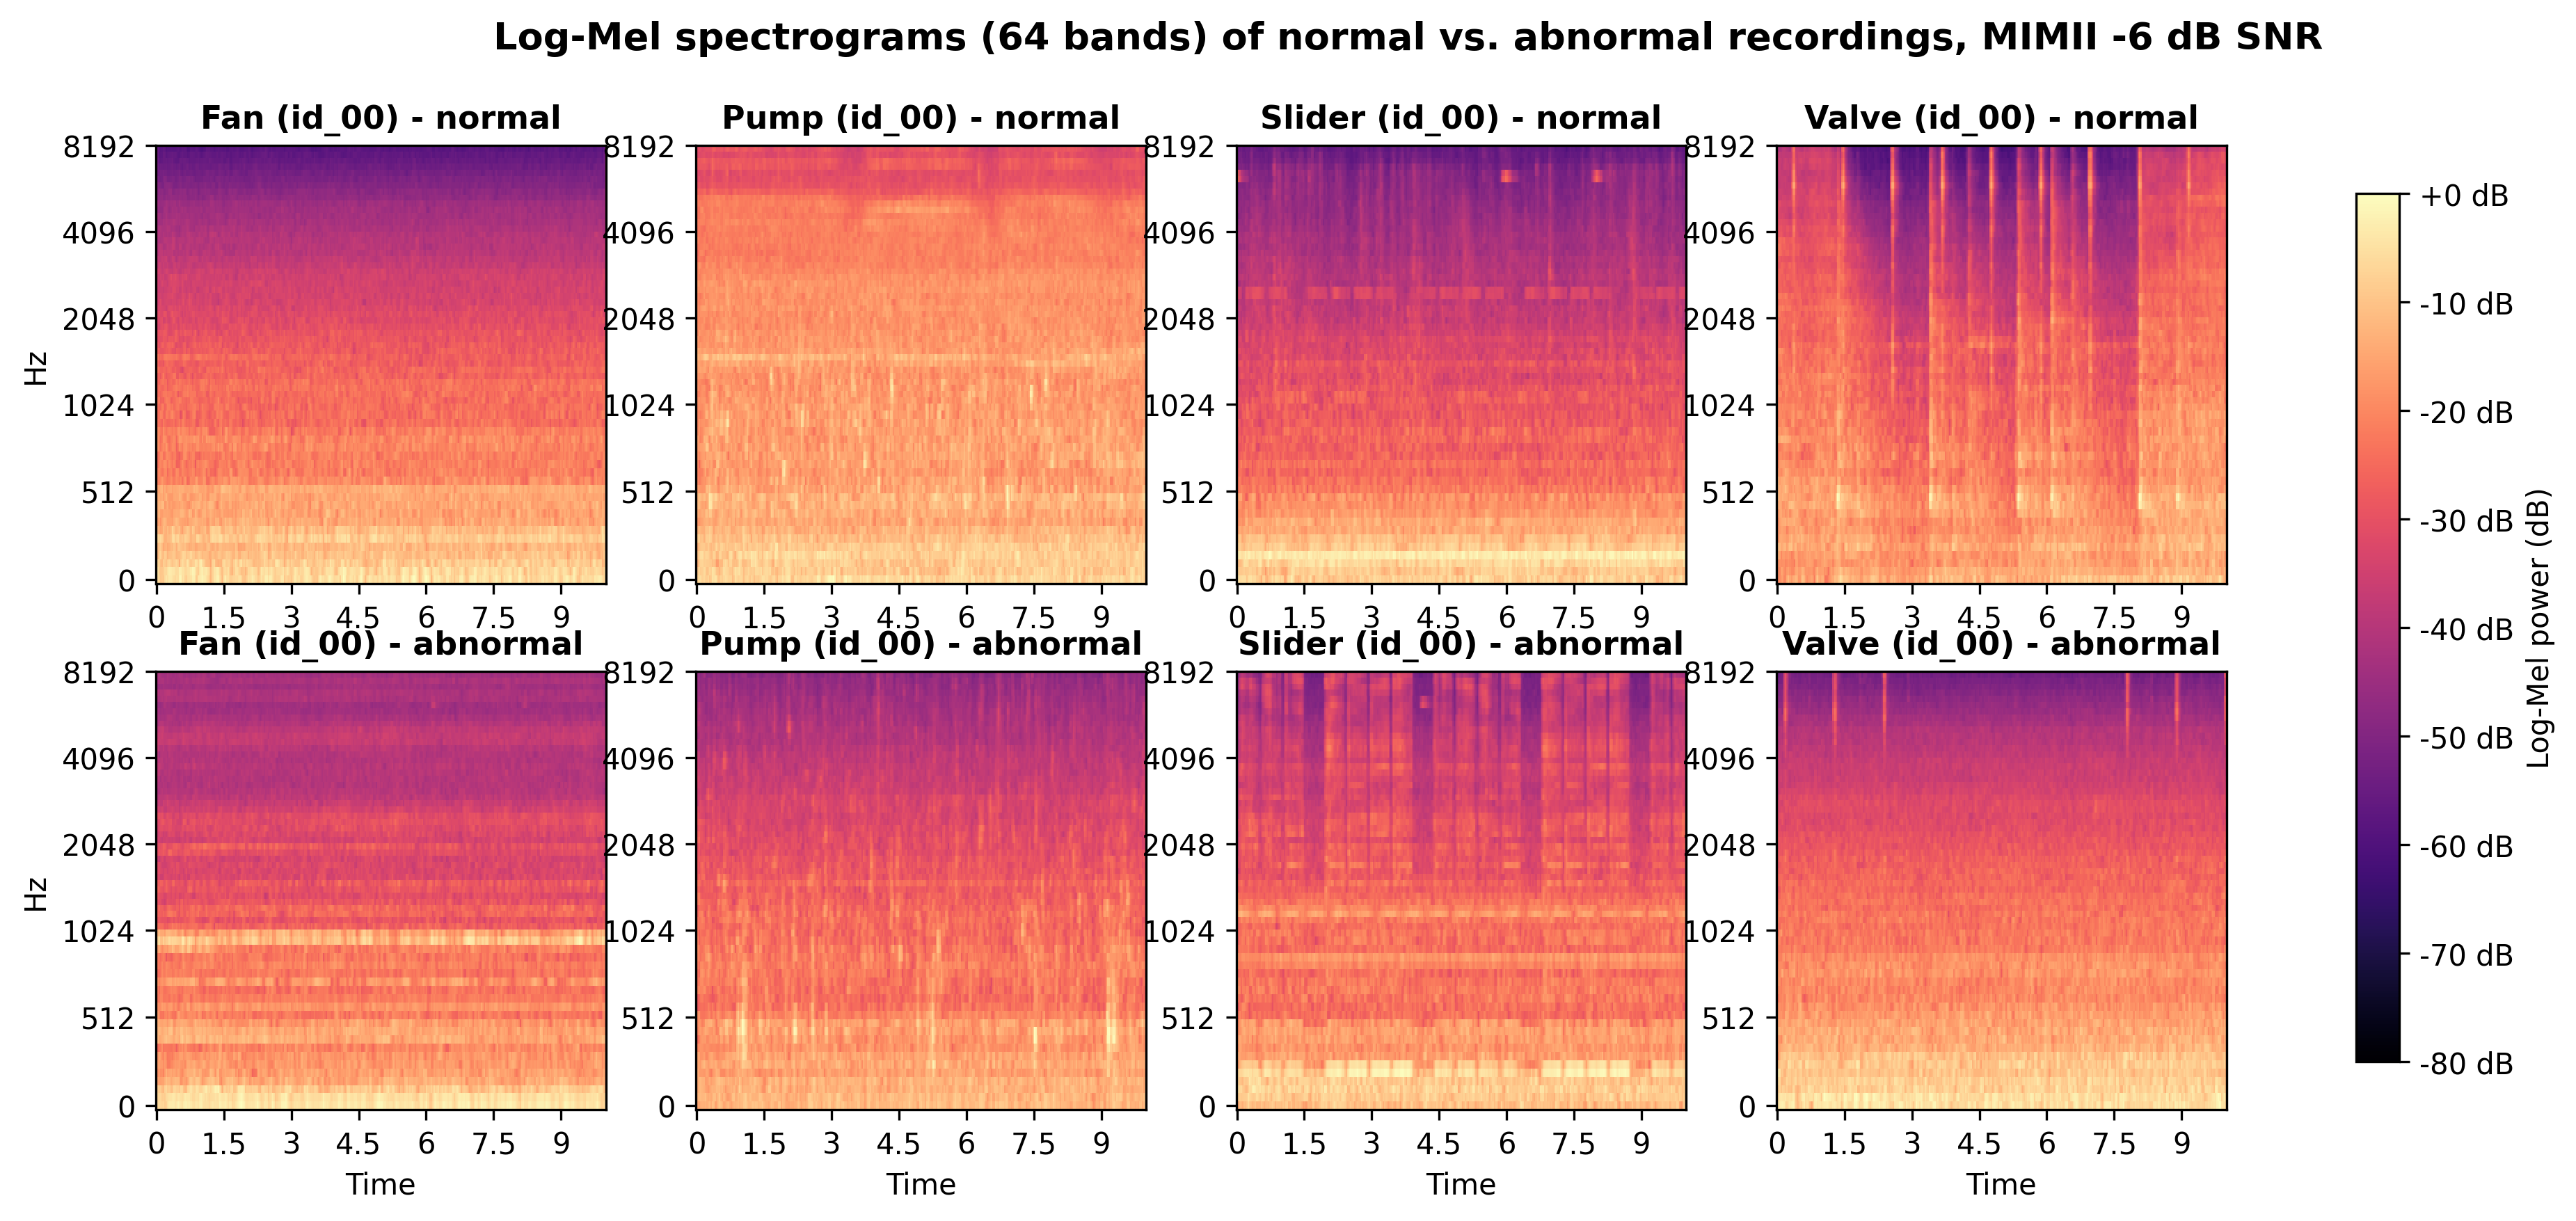
\includegraphics[width=\textwidth]{spectrogram_exemplars.png}
\caption{Log-Mel spectrograms (64 bands) of representative normal (top row) and abnormal (bottom row) recordings of the four MIMII machine types at $-6$\,dB SNR.}
\label{fig:spectrograms}
\end{figure*}

\subsection{Network architecture}
\label{sec:architecture}
The proposed model, 3B-FC128 (Fig.~\ref{fig:architecture}), comprises three convolutional blocks---each Conv2d($3\times3$, padding~1) $\rightarrow$ batch normalization~\cite{ioffe2015batchnorm} $\rightarrow$ ReLU $\rightarrow$ $2\times2$ max-pooling---with channel progression $1\!\to\!16\!\to\!32\!\to\!64$, followed by a flattened linear layer of 128 units with ReLU and dropout $p=0.3$~\cite{srivastava2014dropout}, and a single-logit output. With MFCC input $(1,40,400)$ the flattened dimension is $64\times5\times50=16{,}000$ and the parameter count is 2{,}071{,}777; with log-Mel input $(1,64,400)$ the flattened dimension is $64\times8\times50=25{,}600$ and the count is 3{,}300{,}577. Both variants execute comfortably on CPU (Section~\ref{sec:deploy}).

\begin{figure*}[t]
\centering
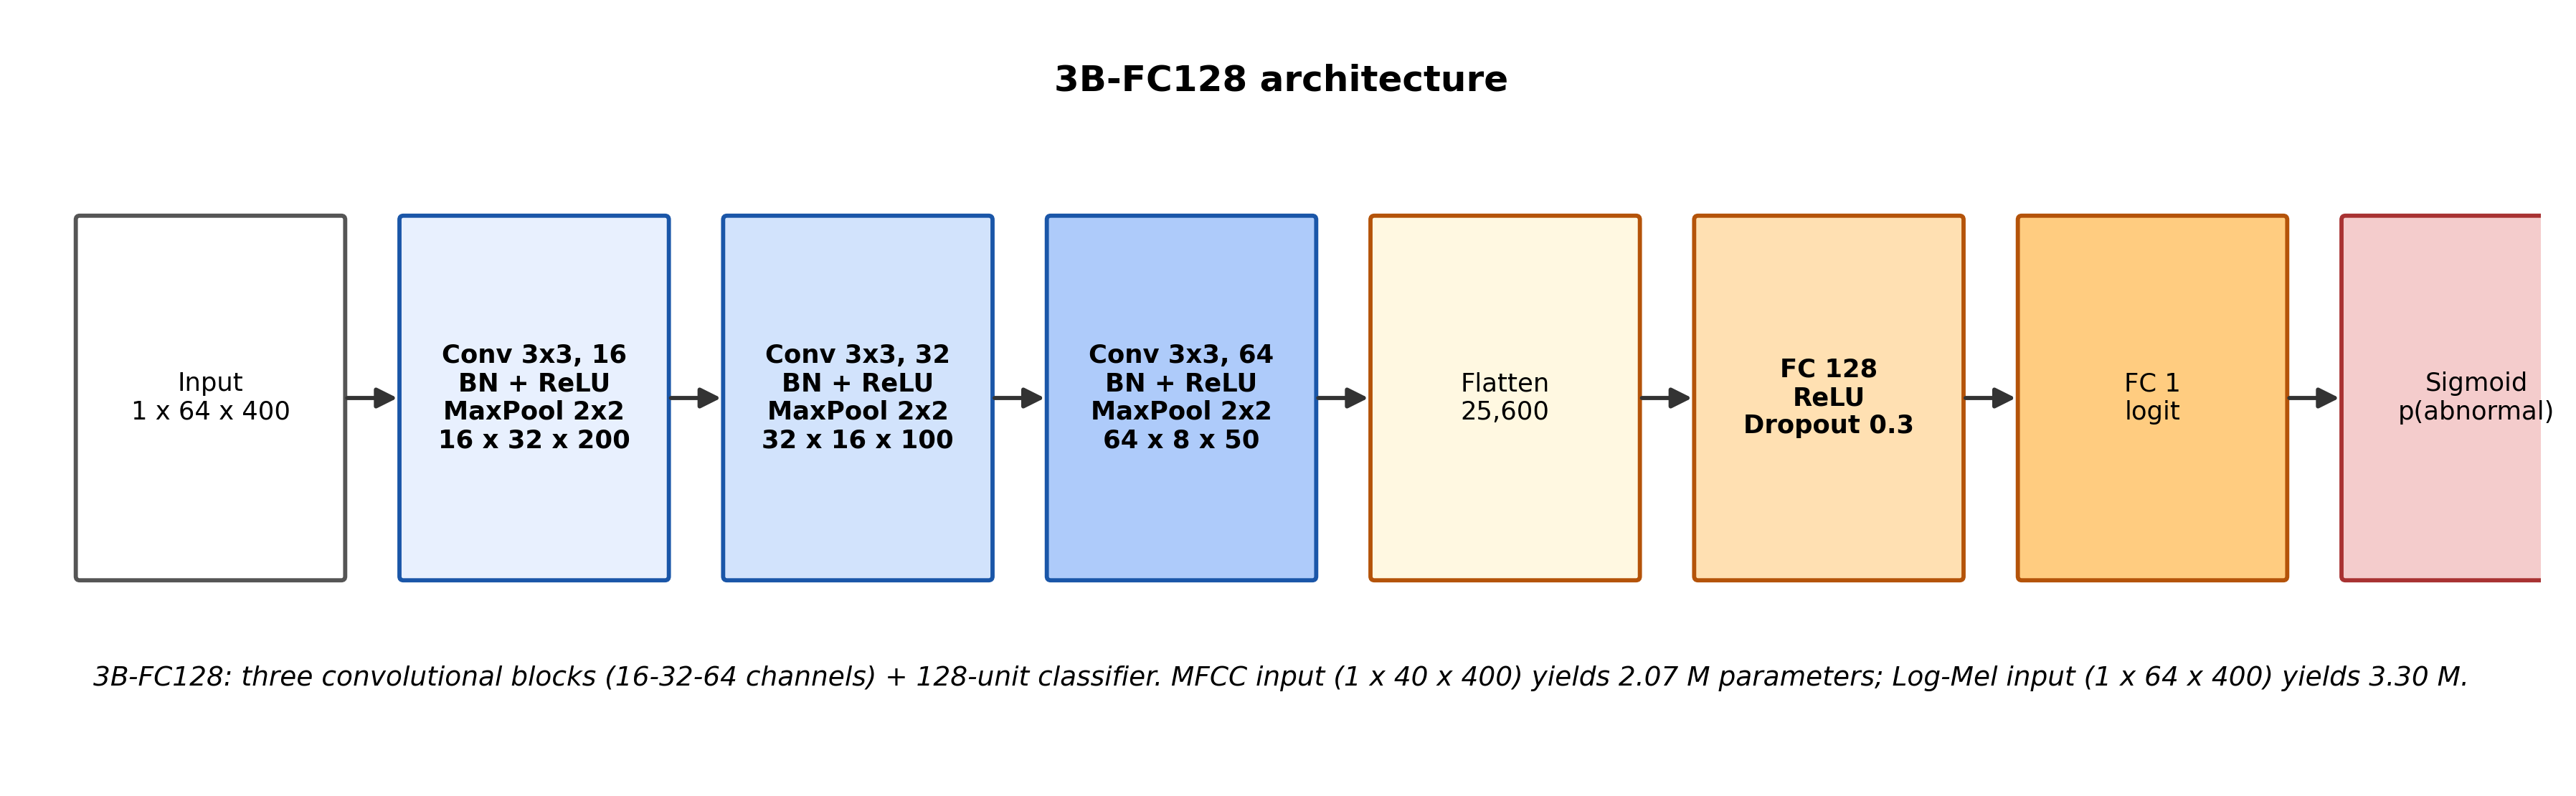
\includegraphics[width=\textwidth]{fig_architecture.png}
\caption{The 3B-FC128 architecture: three convolutional blocks (16--32--64 channels, each with batch normalization, ReLU, and $2\times2$ max-pooling) followed by a 128-unit fully connected classifier with dropout.}
\label{fig:architecture}
\end{figure*}

\subsection{Training configuration}
\label{sec:training}
Independent per-machine models are trained on CPU with AdamW~\cite{loshchilov2019adamw} (learning rate $10^{-4}$, default weight decay $0.01$, PyTorch~\cite{paszke2019pytorch} 2.12), batch size 32, and 10 epochs. The loss is binary cross-entropy with logits; in class-weighted configurations the positive-class weight equals the per-machine normal-to-abnormal ratio (fan 2.8, pump 8.2, slider 3.6, valve 7.7), so a missed abnormal sample incurs proportionally larger loss and the trivial all-normal solution is penalized.

In the single-seed ablations of Sections~\ref{sec:collapse}--\ref{sec:arch}, the seed fixes only the train/test partition, via the generator used for the 80/20 split; network weight initialization and training-batch order draw on the global RNG and are not separately seeded in these exploratory runs. Consequently, nominally identical single-seed configurations evaluated by different ablation scripts can diverge despite an identical data partition, and this affects every machine to some degree, not only the valve: the unweighted MFCC baseline of Table~\ref{tab:baseline} and the unweighted (``B'') rows of Table~\ref{tab:posweight} are both nominally ``MFCC, unweighted, seed 42,'' yet AUC differs by up to 0.02 for fan, pump, and slider and from 0.7366 to 0.7747 for the valve, despite identical accuracy/precision/recall/F1 for the latter. The effect is far larger under class-weighted loss, where the valve category is, as Section~\ref{sec:multiseed} demonstrates, highly sensitive to initialization and training trajectory under 7.7:1 imbalance: nominally identical weighted MFCC seed-42 runs diverge from 0.50 to 0.94 across Tables~\ref{tab:posweight}, \ref{tab:representation}, and \ref{tab:arch}. The ten-seed protocol below (Section~\ref{sec:protocol}) seeds both the partition and the initialization identically per seed (\texttt{torch.manual\_seed} and \texttt{numpy.random.seed}, in addition to the split generator) and is the sole basis for every confirmatory claim in this paper; single-seed ablation values throughout Sections~\ref{sec:collapse}--\ref{sec:arch} are illustrative only and should not be compared across tables at face value.

\subsection{Evaluation protocol}
\label{sec:protocol}
Metrics are AUC--ROC; partial AUC (pAUC) at $\mathrm{FPR}\le0.1$, the low-false-positive region relevant in practice and standard in DCASE evaluation~\cite{koizumi2020dcase}; and accuracy, precision, recall, and F1, all computed with scikit-learn~\cite{pedregosa2011scikitlearn}. Threshold-dependent metrics are reported both at the conventional threshold 0.5 and at a calibrated threshold $\tau^\ast$ chosen to maximize F1 on the \emph{training-set} precision--recall curve (the test set is never used for calibration).

The headline protocol repeats training and evaluation over ten seeds $\{42, 0, 123, 456, 789, 1, 2024, 999, 7, 314\}$, redrawing the 80/20 partition and the initialization per seed, and reports mean $\pm$ standard deviation with 95\% bootstrap confidence intervals (1{,}000 resamples, SciPy~\cite{virtanen2020scipy}) over the per-seed metrics. Paired representation comparisons (log-Mel vs.\ MFCC) are assessed with a one-sided Wilcoxon signed-rank test (SciPy~\cite{virtanen2020scipy}) on the matched per-seed AUCs. Single-seed results are presented only for ablation context and are explicitly labelled as such, because Section~\ref{sec:collapse} shows that single-run results for the most imbalanced category are not stable across seeds.

\subsection{Autoencoder baseline}
\label{sec:ae-method}
To anchor the comparison with the unsupervised paradigm under identical data handling, a convolutional autoencoder was trained per machine type on normal training samples only (20 epochs, learning rate $10^{-3}$, batch 32), scoring test samples by mean-squared reconstruction error. This reproduction complements the published MIMII autoencoder baseline ($\approx0.64$ average AUC at $-6$\,dB~\cite{purohit2019mimii}).

\subsection{Leave-one-machine-ID-out cross-validation}
\label{sec:lomo-method}
To measure generalization to unseen machine \emph{units} of the same model, leave-one-machine-ID-out (LOMO) cross-validation trains on three of the four machine identifiers and tests on the held-out identifier, rotating over all four. This stresses the domain shift dimension emphasized by DCASE 2021--2022~\cite{kawaguchi2021dcase,dohi2022dcase} at the unit level (not across machine types). LOMO is run with the proposed log-Mel + class-weighted configuration for all four machine types, so the generalization analysis is consistent with the proposed model.

% ==================================================================
\section{Detection results}
\label{sec:results}

\subsection{Baseline behaviour and decision collapse under imbalance}
\label{sec:collapse}

Table~\ref{tab:baseline} reports the single-seed (42) baseline with MFCC input and unweighted loss. Fan, pump, and slider attain AUCs of 0.90--0.97, far above the $\approx0.64$ autoencoder reference, confirming the advantage of supervised discrimination at $-6$\,dB. The valve category, however, exhibits a pathological outcome: nominal accuracy of 86.93\% with precision, recall, and F1 all equal to zero. The confusion matrix (TN~$=725$, FP~$=0$, FN~$=109$, TP~$=0$; Fig.~\ref{fig:confusion}) shows that every test sample is assigned to the normal class: the classifier has collapsed onto the majority-class prior. The AUC of 0.7366 despite collapse indicates that the model's continuous scores still rank abnormal samples somewhat higher than normal ones, but the entire score distribution lies below the 0.5 decision threshold---a ``soft collapse'' in which learned logit offsets cannot overcome the prior induced by the unweighted loss under 7.7:1 imbalance.

\begin{table}[t]
\centering
\caption{Single-seed baseline (seed 42): MFCC input, unweighted loss, $-6$\,dB, 80/20 split.}
\label{tab:baseline}
\setlength{\tabcolsep}{4pt}
\begin{tabular}{lcccccc}
\toprule
Machine & Acc.\,(\%) & Prec. & Recall & F1 & AUC & $N_\mathrm{test}$ \\
\midrule
Fan    & 85.86 & 0.7599 & 0.7333 & 0.7464 & 0.9011 & 1{,}110 \\
Pump   & 95.72 & 0.8909 & 0.6203 & 0.7313 & 0.9445 & 841 \\
Slider & 95.12 & 0.9839 & 0.7625 & 0.8592 & 0.9730 & 819 \\
Valve  & 86.93 & 0.0000 & 0.0000 & 0.0000 & 0.7366 & 834 \\
\bottomrule
\end{tabular}
\end{table}

\begin{figure}[t]
\centering
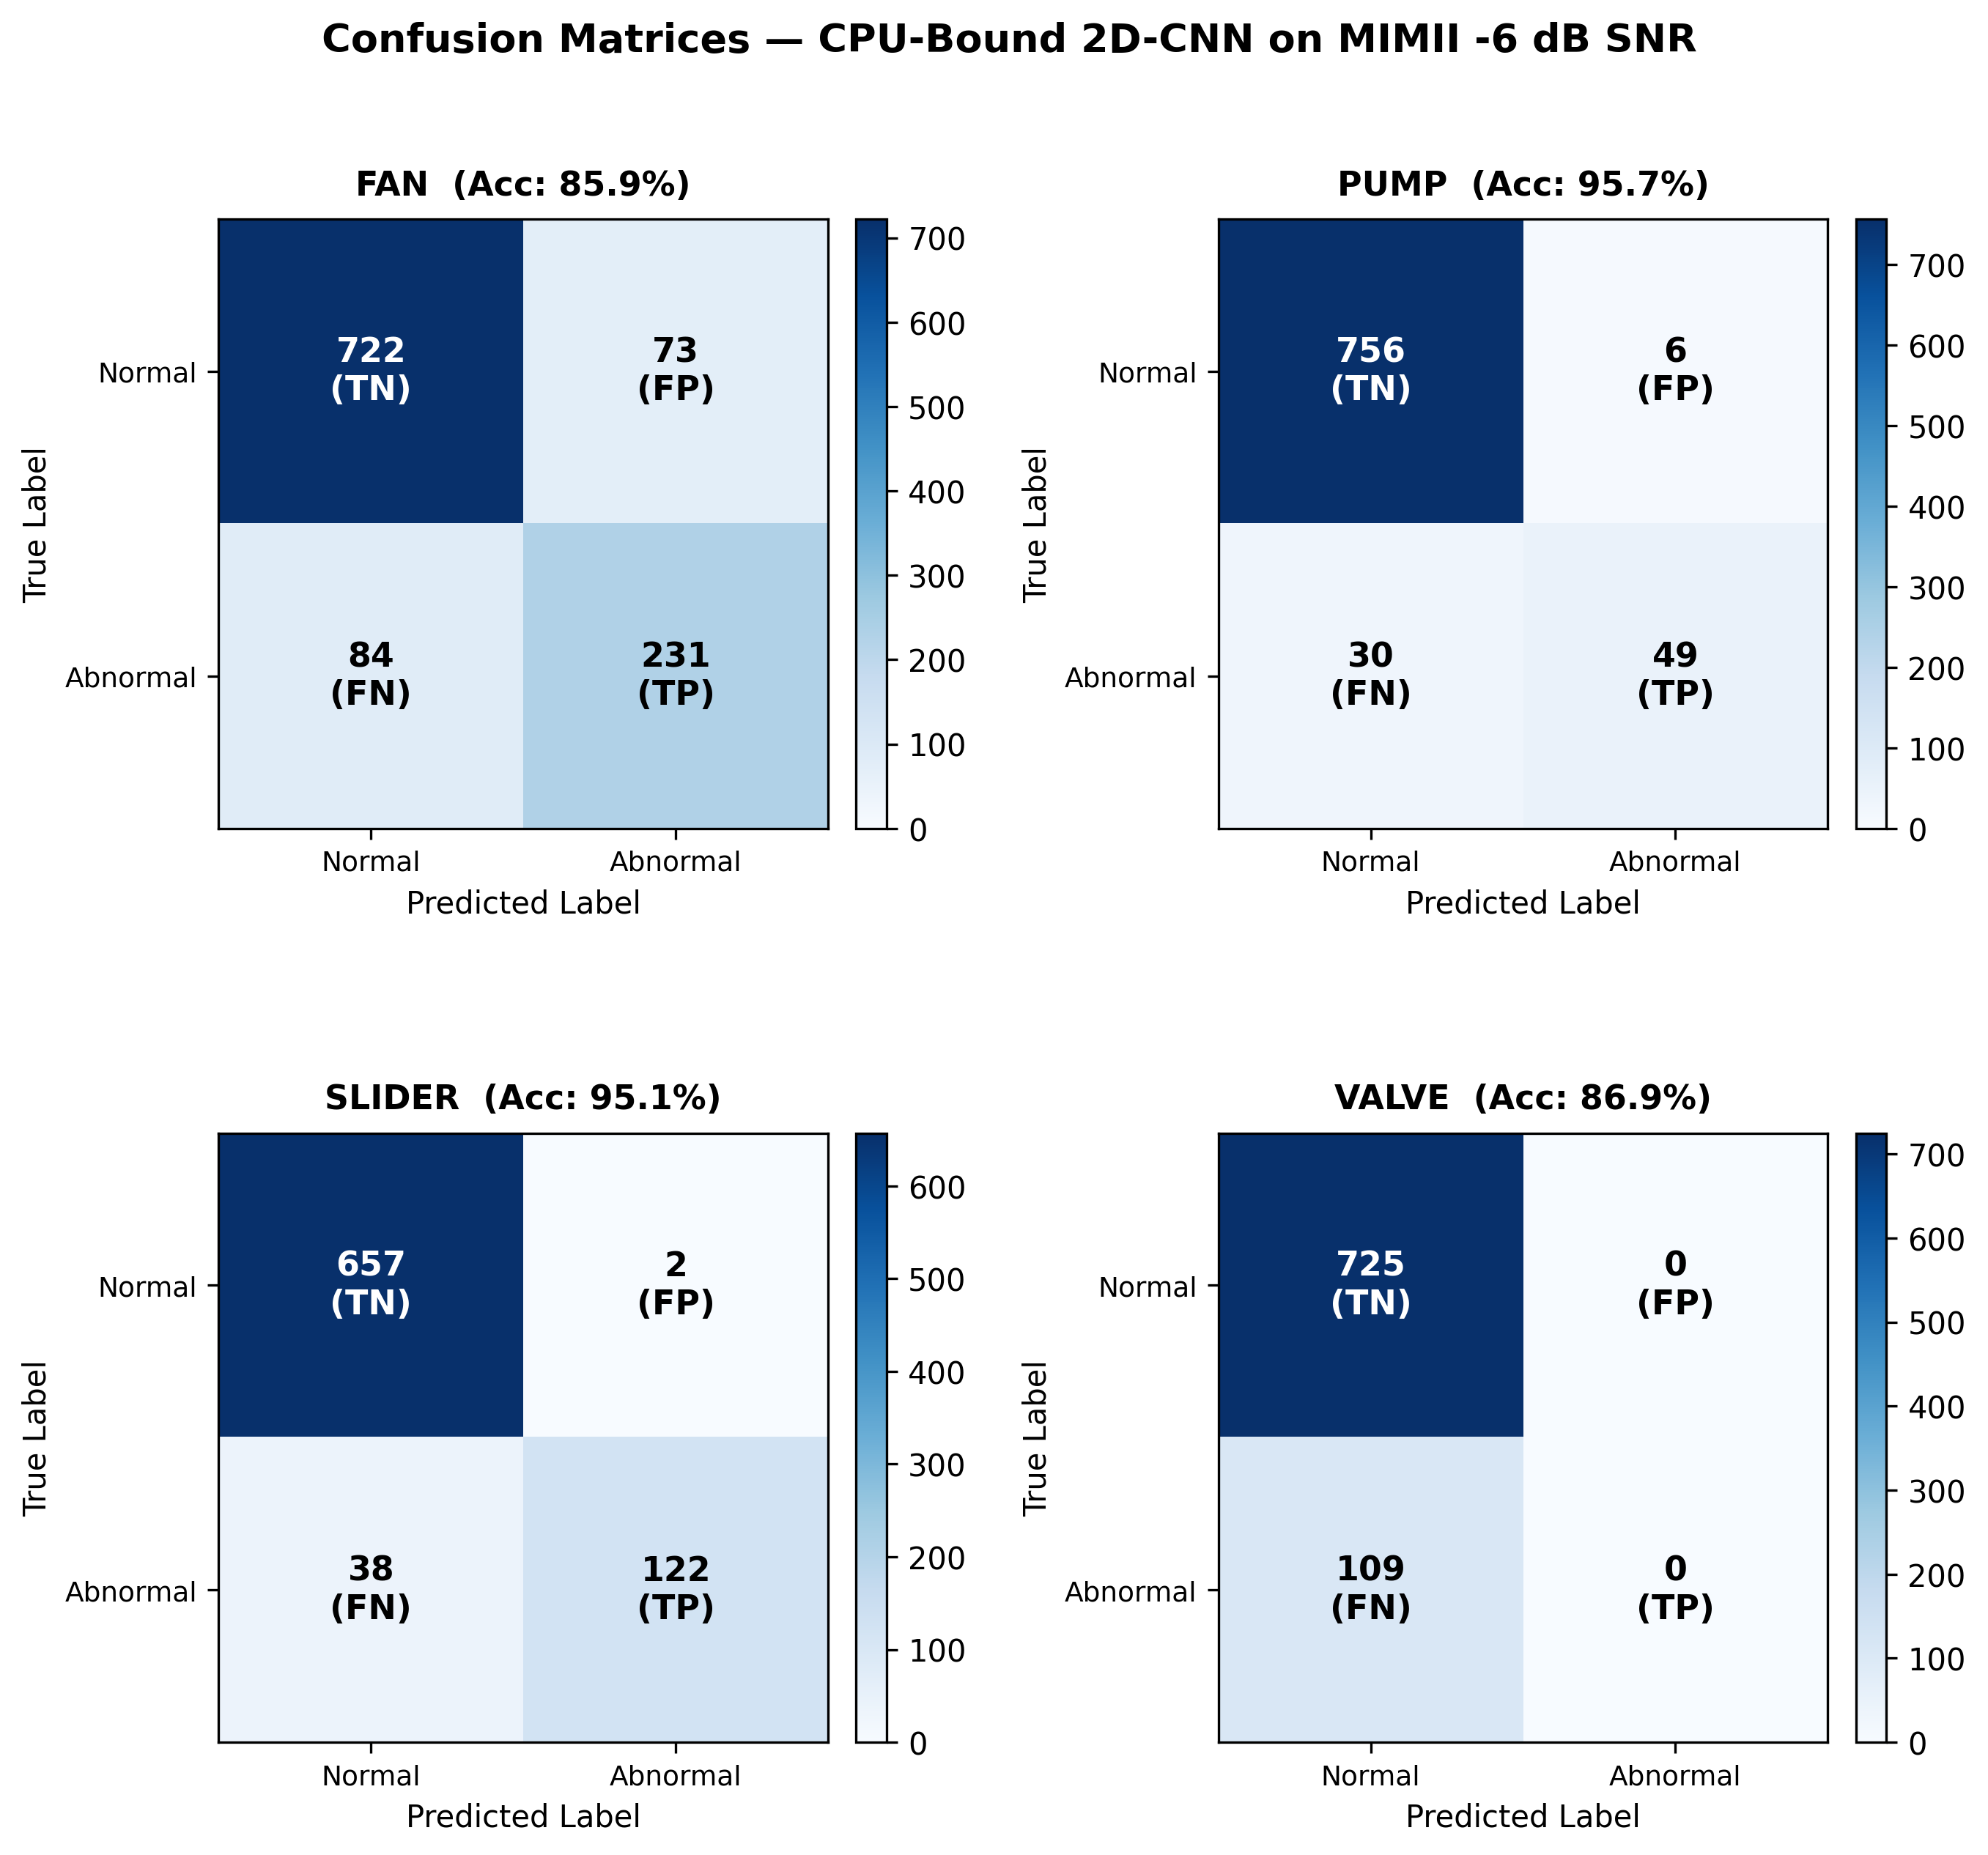
\includegraphics[width=\columnwidth]{confusion_matrices.png}
\caption{Confusion matrices for the MFCC/unweighted baseline at $-6$\,dB (seed 42). The valve panel shows zero true positives: complete decision collapse.}
\label{fig:confusion}
\end{figure}

\begin{figure}[t]
\centering
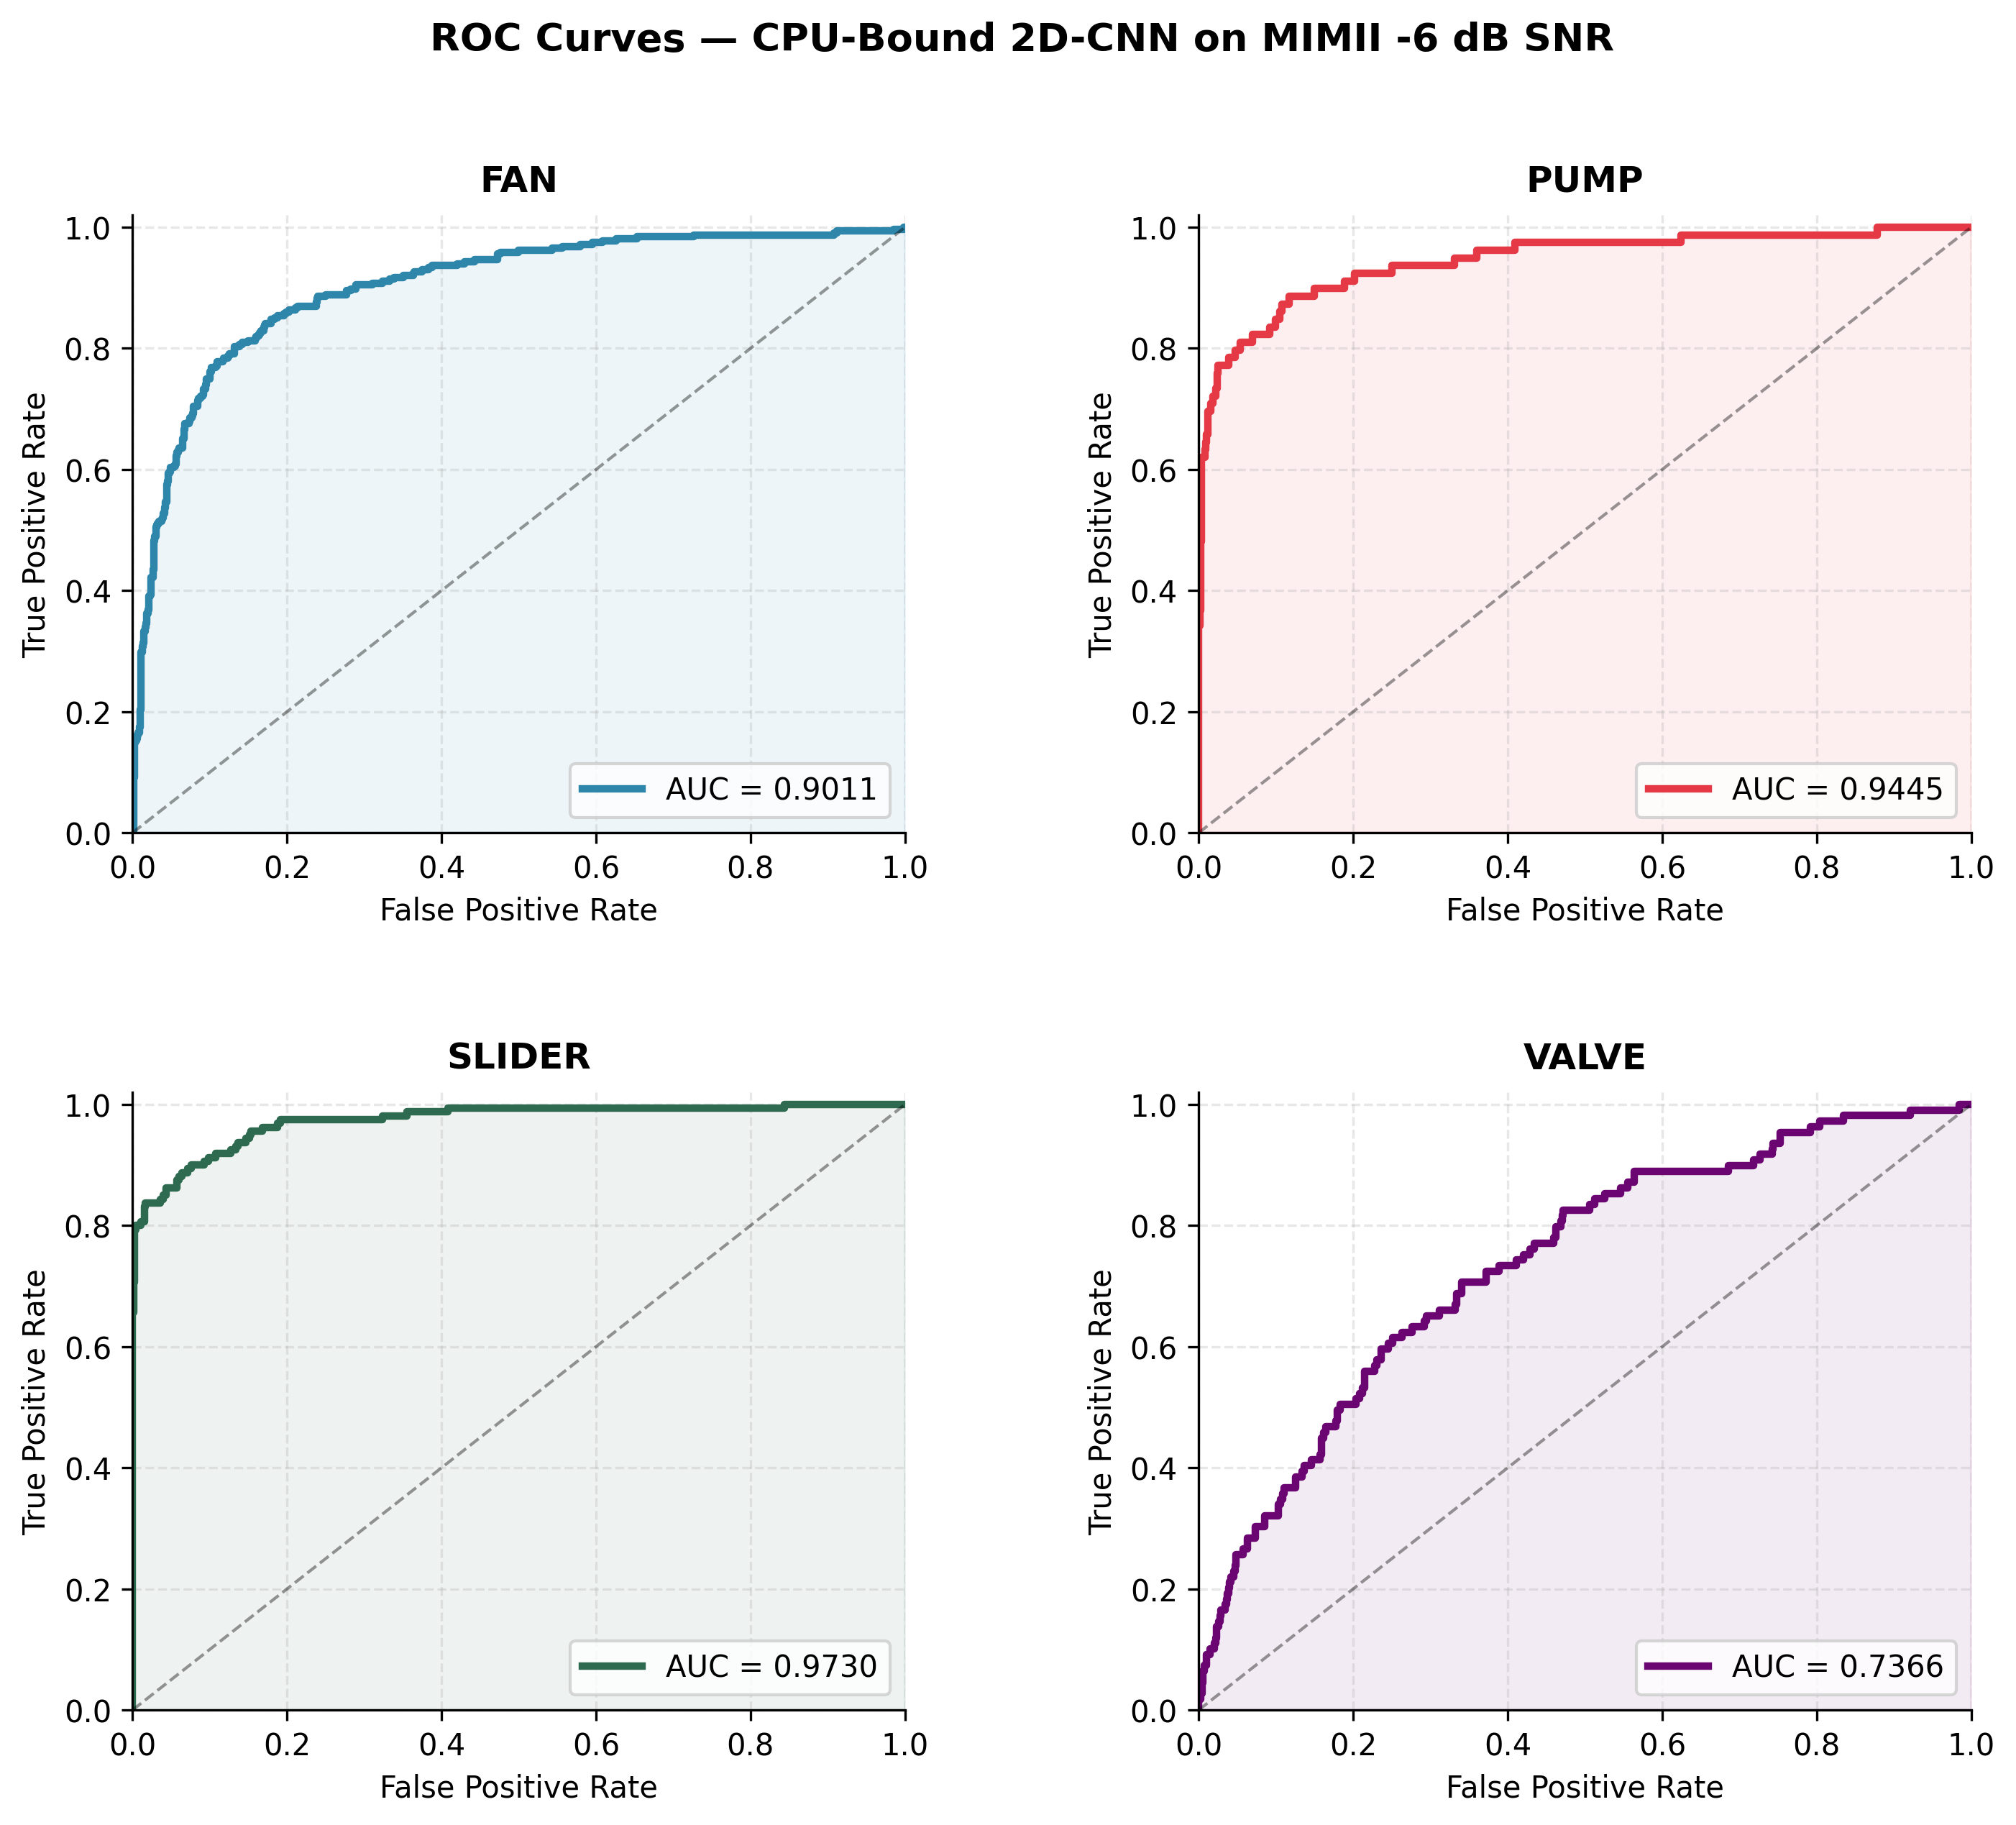
\includegraphics[width=\columnwidth]{roc_curves.png}
\caption{ROC curves for the MFCC/unweighted baseline (seed 42). The valve curve has non-trivial area (0.7366) yet yields zero sensitivity at the 0.5 operating point.}
\label{fig:roc}
\end{figure}

Training convergence (Fig.~\ref{fig:convergence}) corroborates this interpretation: valve training loss decreases monotonically while validation loss plateaus, consistent with optimization settling into the majority-class minimum rather than overfitting.

\begin{figure}[t]
\centering
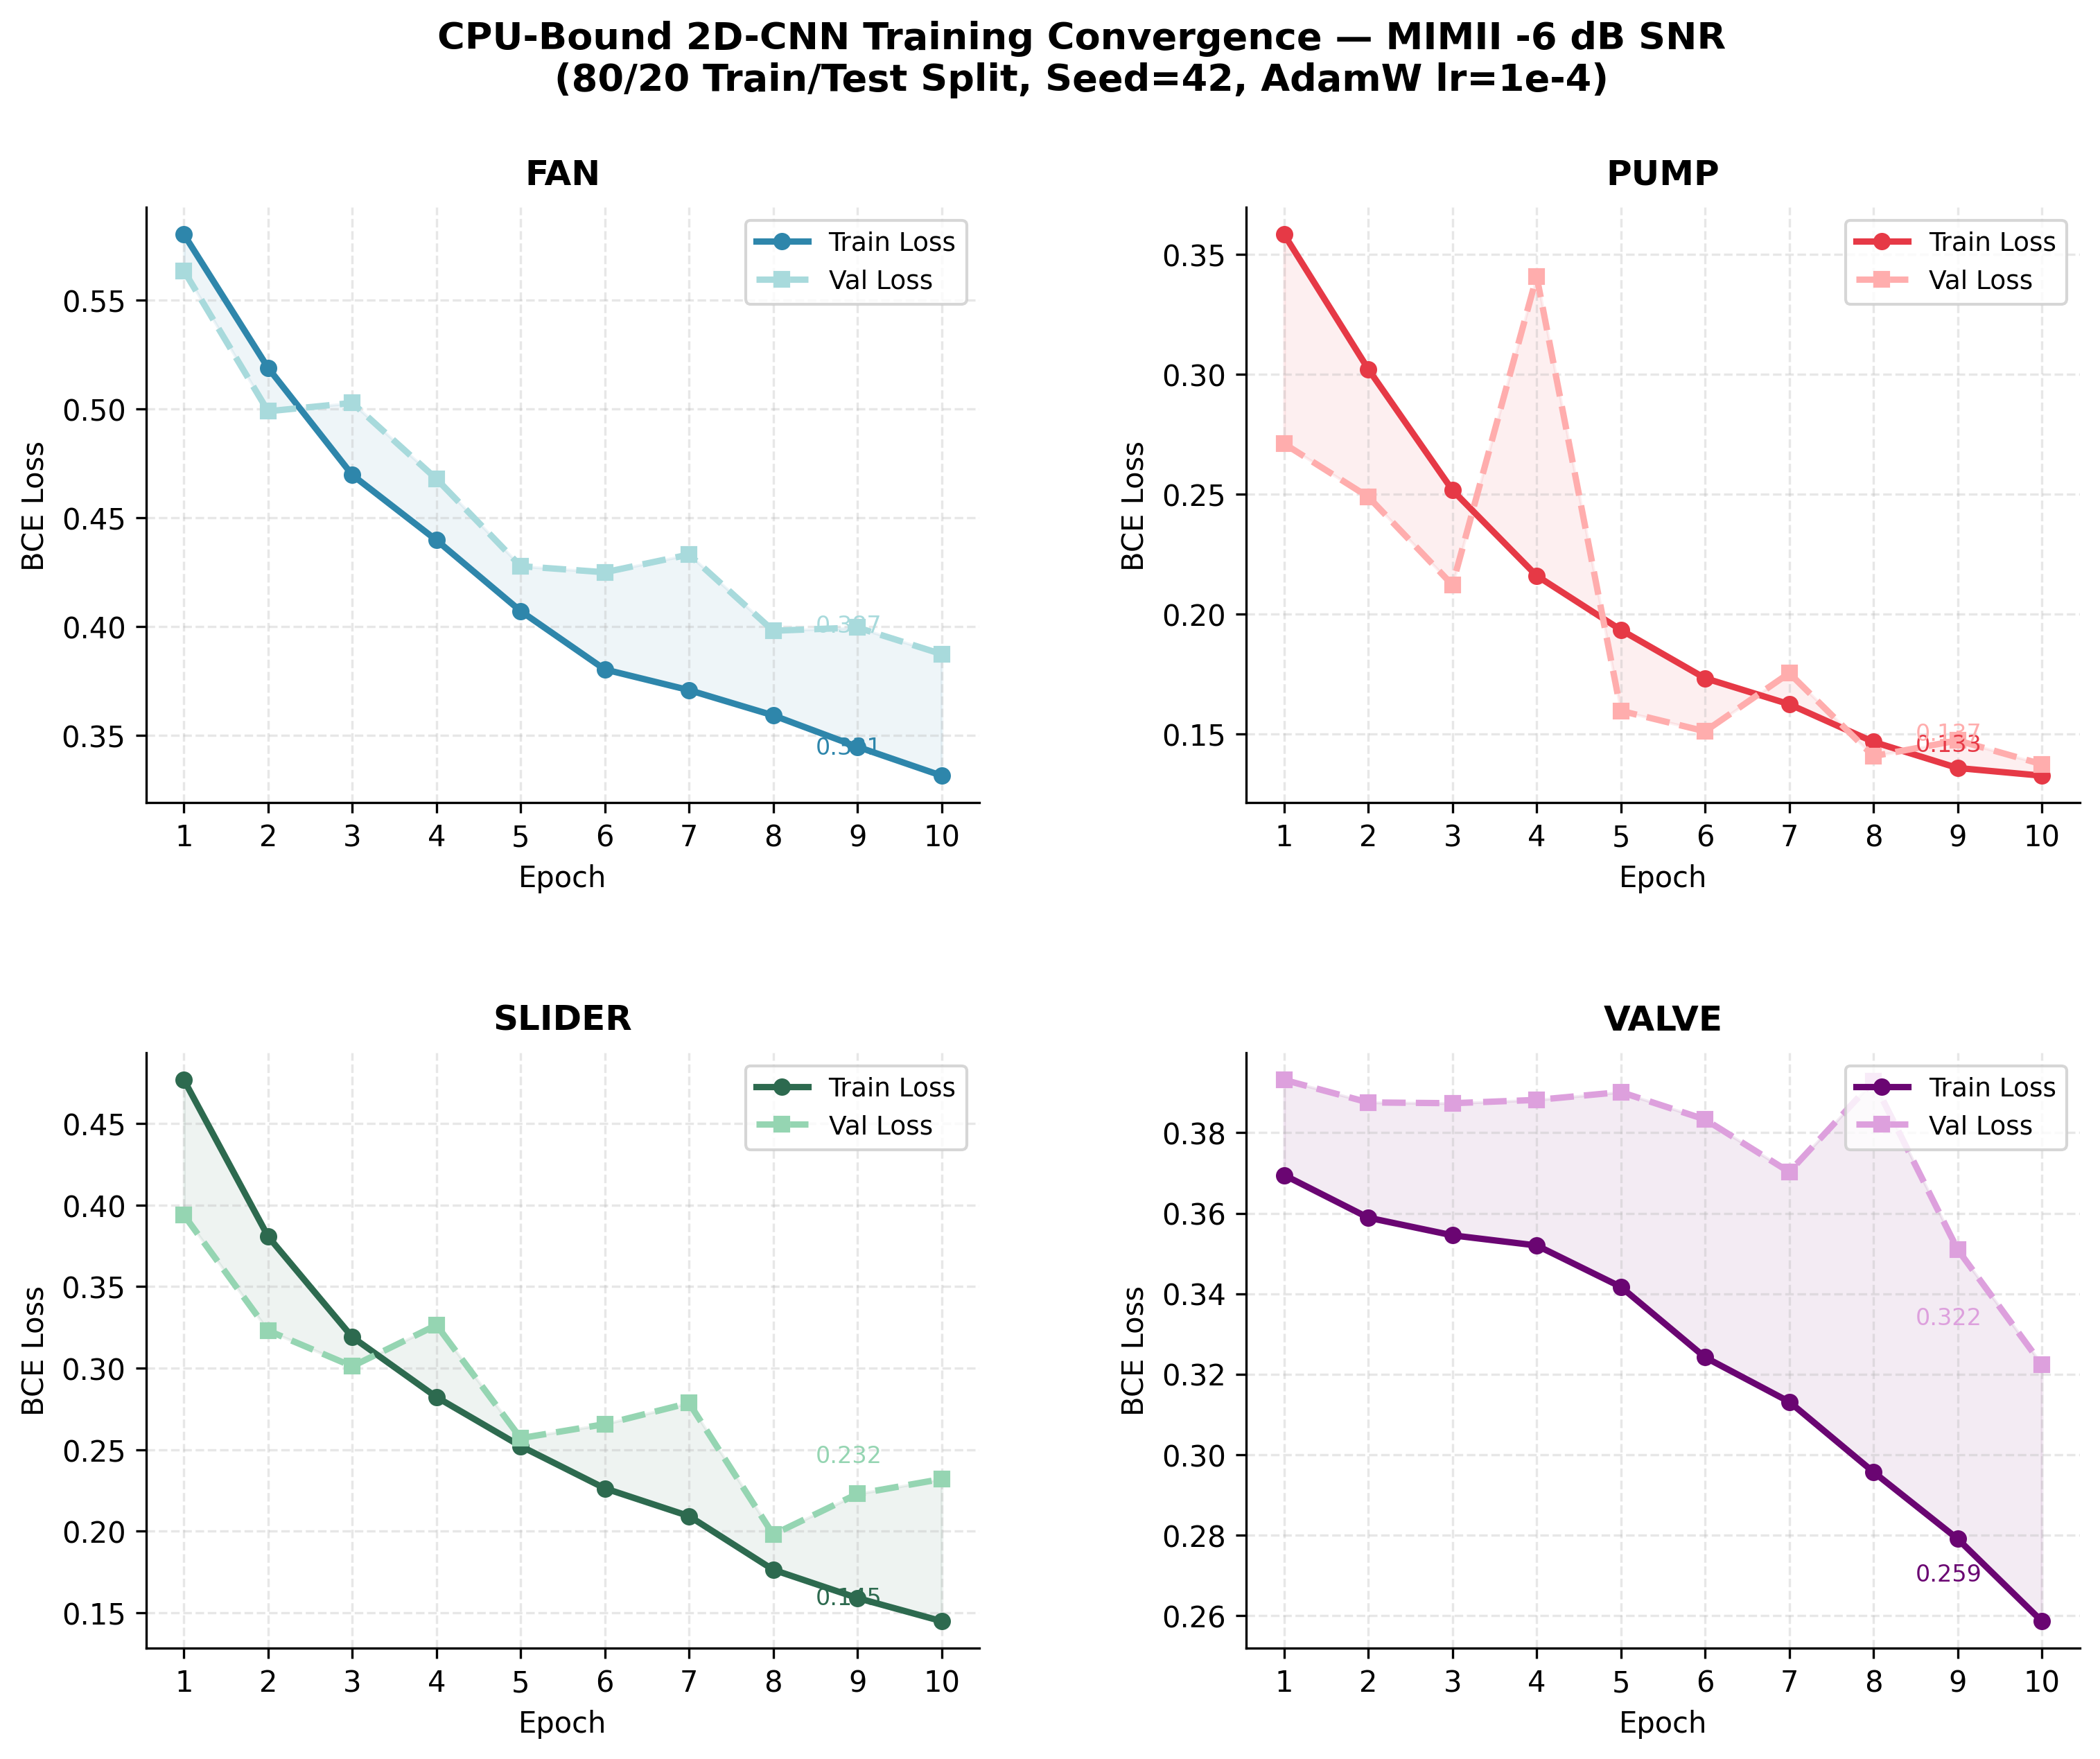
\includegraphics[width=\columnwidth]{training_convergence.png}
\caption{Training and validation loss over 10 epochs (MFCC, unweighted, seed 42).}
\label{fig:convergence}
\end{figure}

\subsection{Re-weighting alone does not repair the valve category}
\label{sec:posweight}

Applying the class-weighted loss to MFCC input shifts all four operating points toward recall, as expected (Table~\ref{tab:posweight}): fan recall rises from 0.63 to 0.86 and slider remains strong. For the valve, re-weighting alone produces only partial, low-quality recovery in this run (F1 $=0.32$, AUC $=0.74$), and in repeated runs frequently no recovery at all (Section~\ref{sec:multiseed}): the representation, not only the loss, is implicated.

\begin{table}[t]
\centering
\caption{Effect of class-weighted loss with MFCC input (seed 42). ``B''/``W'' denote unweighted and weighted loss.}
\label{tab:posweight}
\setlength{\tabcolsep}{3.5pt}
\begin{tabular}{llccccc}
\toprule
Machine & Loss & Acc.\,(\%) & Prec. & Recall & F1 & AUC \\
\midrule
Fan    & B & 83.60 & 0.7509 & 0.6317 & 0.6862 & 0.9010 \\
       & W & 78.56 & 0.5832 & 0.8571 & 0.6941 & 0.8864 \\
Pump   & B & 94.89 & 0.8000 & 0.6076 & 0.6906 & 0.9300 \\
       & W & 71.58 & 0.2368 & 0.9114 & 0.3760 & 0.9265 \\
Slider & B & 93.77 & 0.9739 & 0.7000 & 0.8145 & 0.9634 \\
       & W & 93.41 & 0.8354 & 0.8250 & 0.8302 & 0.9577 \\
Valve  & B & 86.93 & 0.0000 & 0.0000 & 0.0000 & 0.7747 \\
       & W & 80.94 & 0.3016 & 0.3486 & 0.3234 & 0.7421 \\
\bottomrule
\end{tabular}
\end{table}

\subsection{Spectral representation is the decisive factor}
\label{sec:representation}

Table~\ref{tab:representation} compares MFCC and log-Mel inputs under identical class-weighted training (seed 42). For fan, pump, and slider the two representations are comparable, with log-Mel slightly ahead (mean AUC 0.9378 vs.\ 0.8315 is dominated by the valve difference). For the valve, MFCC remains fully collapsed (AUC $=0.500$, F1 $=0$) while log-Mel reaches AUC $=0.8877$ with F1 $=0.5136$.

\begin{table}[t]
\centering
\caption{Representation ablation under class-weighted loss (seed 42).}
\label{tab:representation}
\setlength{\tabcolsep}{3.5pt}
\begin{tabular}{llcccc}
\toprule
Input & Machine & AUC & F1 & Recall & Acc.\,(\%) \\
\midrule
MFCC (40)
 & Fan    & 0.9023 & 0.7372 & 0.7968 & 83.87 \\
 & Pump   & 0.9465 & 0.6782 & 0.7468 & 93.34 \\
 & Slider & 0.9770 & 0.7260 & 0.9688 & 85.71 \\
 & Valve  & 0.5000 & 0.0000 & 0.0000 & 86.93 \\
 & \emph{Mean AUC} & 0.8315 & & & \\
\midrule
Log-Mel (64)
 & Fan    & 0.9075 & 0.7251 & 0.6825 & 85.32 \\
 & Pump   & 0.9687 & 0.7667 & 0.8734 & 95.01 \\
 & Slider & 0.9874 & 0.9121 & 0.8750 & 96.70 \\
 & Valve  & 0.8877 & 0.5136 & 0.6055 & 85.01 \\
 & \emph{Mean AUC} & 0.9378 & & & \\
\bottomrule
\end{tabular}
\end{table}

\begin{figure}[t]
\centering
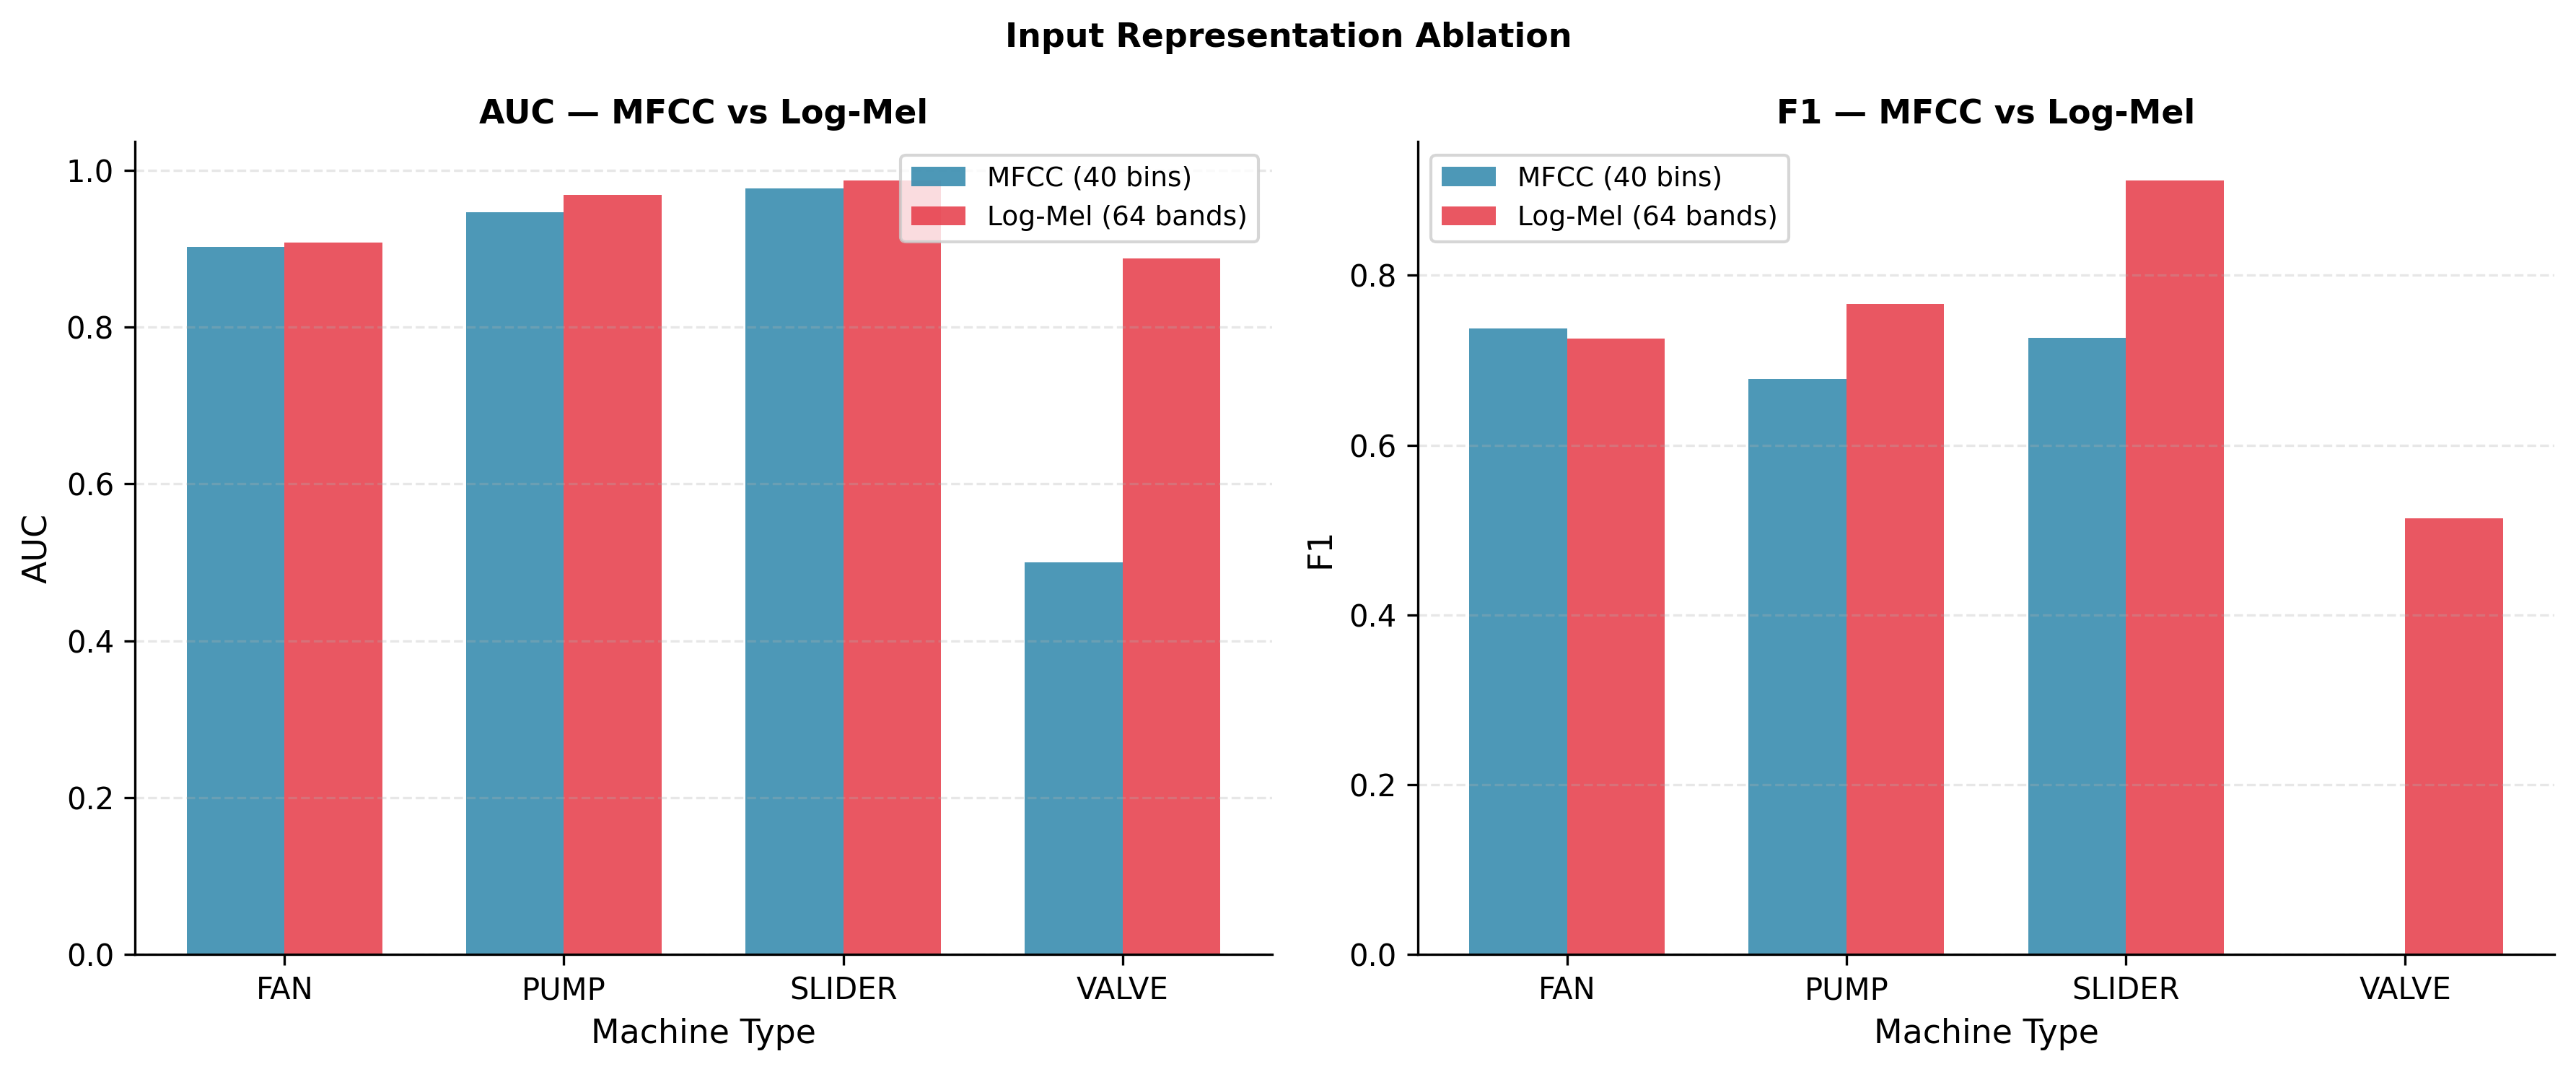
\includegraphics[width=\columnwidth]{representation_ablation_plot.png}
\caption{AUC (left) and F1 (right) for MFCC versus log-Mel input under class-weighted loss.}
\label{fig:representation}
\end{figure}

A plausible mechanism, grounded in the signal processing rather than directly measured here, is as follows. Valve anomalies (seal degradation, blockage) produce broadband, transient spectral perturbations that span multiple Mel bands simultaneously. The DCT in MFCC computation compacts each frame onto a small set of decorrelated cepstral coefficients, which by construction reduces inter-band correlation and could plausibly discard co-occurrence structure that distinguishes these transients from the (likewise broadband) factory noise floor. The log-Mel representation preserves the full band-energy topology, allowing the convolutional layers to learn localized spectro-temporal anomaly signatures. We did not directly verify this mechanism (e.g.\ via feature correlation analysis or ablation isolating the DCT step in isolation); the claim rests on the observed performance gap together with the established signal-processing property of the DCT, and should be read as a hypothesis consistent with the data rather than a demonstrated causal account. This comparison is deliberately bounded to the two most widely used inputs---cepstral MFCC and filterbank log-Mel---and the ``decisive'' claim should be read within that scope; psychoacoustically motivated or learned representations~\cite{wissbrock2024more} may yield further gains and are left to future work. The configuration \emph{log-Mel + class-weighted loss + 3B-FC128} is therefore designated the proposed configuration for all subsequent analysis.

\subsection{Multi-seed validation of the proposed configuration}
\label{sec:multiseed}

Single-run valve results are not trustworthy: across ten seeds of the \emph{MFCC} + weighted configuration, valve AUC ranges from 0.49 to 0.81 (mean $0.616\pm0.112$) and F1 from 0.00 to 0.44, i.e.\ the category collapses on six of ten seeds. This bimodal instability---to our knowledge unreported for MIMII valve---implies that any single-seed valve claim, favourable or not, conveys little information, and motivates the protocol of Section~\ref{sec:protocol}.

Table~\ref{tab:multiseed} reports the ten-seed statistics of the proposed configuration. Three results stand out. First, log-Mel input improves the mean AUC of \emph{every} machine type relative to the MFCC + weighted configuration under identical seeds: fan $0.9039\!\to\!0.9408$, pump $0.9345\!\to\!0.9452$, slider $0.9696\!\to\!0.9883$, and valve $0.6160\!\to\!0.9624$. A one-sided Wilcoxon signed-rank test over the ten paired seeds, run independently per machine to avoid pooling non-exchangeable observations across distinct machine populations, confirms that this improvement is statistically significant for every machine type (fan, slider, and valve $p=0.001$; pump $p=0.014$), though with four per-machine tests a conservative Bonferroni correction ($\alpha=0.05/4=0.0125$) would leave the pump result marginal while fan, slider, and valve remain comfortably significant; log-Mel wins on 38 of 40 seed--machine pairs overall. Second, and most importantly, the valve recovery is \emph{robust}: no seed collapses (per-seed AUC ranges from 0.9115 to 0.9912, 95\% bootstrap CI $[0.945, 0.976]$), whereas the MFCC configuration collapsed on six of ten seeds. The residual valve variance is concentrated in the threshold-dependent metrics (F1 from 0.47 to 0.87 across seeds), reflecting seed-dependent score calibration rather than ranking quality. Third, train-set threshold calibration improves mean F1 on every machine (e.g.\ fan $0.758\!\to\!0.791$, valve $0.681\!\to\!0.731$) while reducing its across-seed standard deviation (fan $0.045\!\to\!0.020$, slider $0.045\!\to\!0.011$), i.e.\ calibration converts ranking quality into operating-point quality without touching the test set. Mean pAUC at $\mathrm{FPR}\le0.1$ remains high for slider (0.970) and pump (0.879), indicating usable sensitivity in the low-false-alarm regime that matters for deployment.

\begin{table*}[t]
\centering
\caption{Ten-seed validation of the proposed configuration (log-Mel 64 + class-weighted loss + 3B-FC128) at $-6$\,dB. Mean $\pm$ SD over seeds; 95\% CI is the bootstrap confidence interval (1{,}000 resamples) on the mean AUC; pAUC at $\mathrm{FPR}\le0.1$; F1$_{0.5}$ at threshold 0.5; F1$_{\tau^\ast}$ at the train-calibrated threshold. The MFCC + weighted column shows mean AUC under the same ten seeds for comparison.}
\label{tab:multiseed}
\small
\setlength{\tabcolsep}{4pt}
\begin{tabular}{lcccccc}
\toprule
Machine & AUC & 95\% CI & pAUC & F1$_{0.5}$ & F1$_{\tau^\ast}$ & AUC (MFCC+W) \\
\midrule
Fan    & $\msFanAuc \pm \msFanAucSd$ & \msFanAucCI & \msFanPauc & \msFanFone & \msFanFcal & $0.9039 \pm 0.0082$ \\
Pump   & $\msPumpAuc \pm \msPumpAucSd$ & \msPumpAucCI & \msPumpPauc & \msPumpFone & \msPumpFcal & $0.9345 \pm 0.0179$ \\
Slider & $\msSliderAuc \pm \msSliderAucSd$ & \msSliderAucCI & \msSliderPauc & \msSliderFone & \msSliderFcal & $0.9696 \pm 0.0088$ \\
Valve  & $\msValveAuc \pm \msValveAucSd$ & \msValveAucCI & \msValvePauc & \msValveFone & \msValveFcal & $0.6160 \pm 0.1123$ \\
\bottomrule
\end{tabular}
\end{table*}

% ==================================================================
\section{Ablations, baselines, and generalization}
\label{sec:ablation}

\subsection{Architecture capacity and depth}
\label{sec:arch}

Table~\ref{tab:arch} benchmarks six variants (MFCC input, class-weighted loss, seed 42) spanning two to four blocks and 64--256-unit classifiers; Fig.~\ref{fig:arch} visualizes the AUC--latency trade-off. Three patterns are robust across machines. First, two-block extractors fail on the valve regardless of classifier width (AUC $\le0.53$): the representational bottleneck lies in the convolutional hierarchy, not the classifier. Second, the three-block, 128-unit configuration attains the best mean AUC (0.935 in this run) at 32--35\,ms batch latency. Third, both widening (FC-256) and deepening (four blocks) \emph{reduce} valve AUC (0.79 and 0.63), consistent with majority-class overfitting and excessive temporal downsampling, respectively. Given the valve seed instability documented above, the per-variant valve values should be read as indicative; the orderings of the fan/pump/slider columns, which are seed-stable, support the same architectural conclusion.

\begin{table}[t]
\centering
\caption{Architecture ablation (MFCC input, class-weighted loss, seed 42). Latency is per batch of 16 on the CPU. Per-variant AUC values are single-seed; see Section~\ref{sec:training} for the scope of the seed in these ablations.}
\label{tab:arch}
\footnotesize
\setlength{\tabcolsep}{2pt}
\begin{tabular}{lccccccc}
\toprule
Variant & AUC (Fan) & AUC (Pump) & AUC (Slider) & AUC (Valve) & Mean AUC & Lat.\,(ms) & Params \\
\midrule
2B-FC64  & 0.5000 & 0.9145 & 0.9273 & 0.5000 & 0.710 & 27.0 & 2.05\,M \\
2B-FC128 & 0.8726 & 0.9122 & 0.9515 & 0.5347 & 0.818 & 27.7 & 4.10\,M \\
3B-FC64  & 0.8841 & 0.9174 & 0.9574 & 0.5000 & 0.815 & 32.6 & 1.05\,M \\
\textbf{3B-FC128} & \textbf{0.9068} & \textbf{0.9233} & \textbf{0.9703} & \textbf{0.9386} & \textbf{0.935} & \textbf{33.7} & \textbf{2.07\,M} \\
3B-FC256 & 0.8974 & 0.9485 & 0.9803 & 0.7922 & 0.905 & 33.9 & 4.12\,M \\
4B-FC128 & 0.9284 & 0.9498 & 0.9649 & 0.6305 & 0.868 & 36.4 & 0.92\,M \\
\bottomrule
\end{tabular}
\end{table}

\begin{figure}[t]
\centering
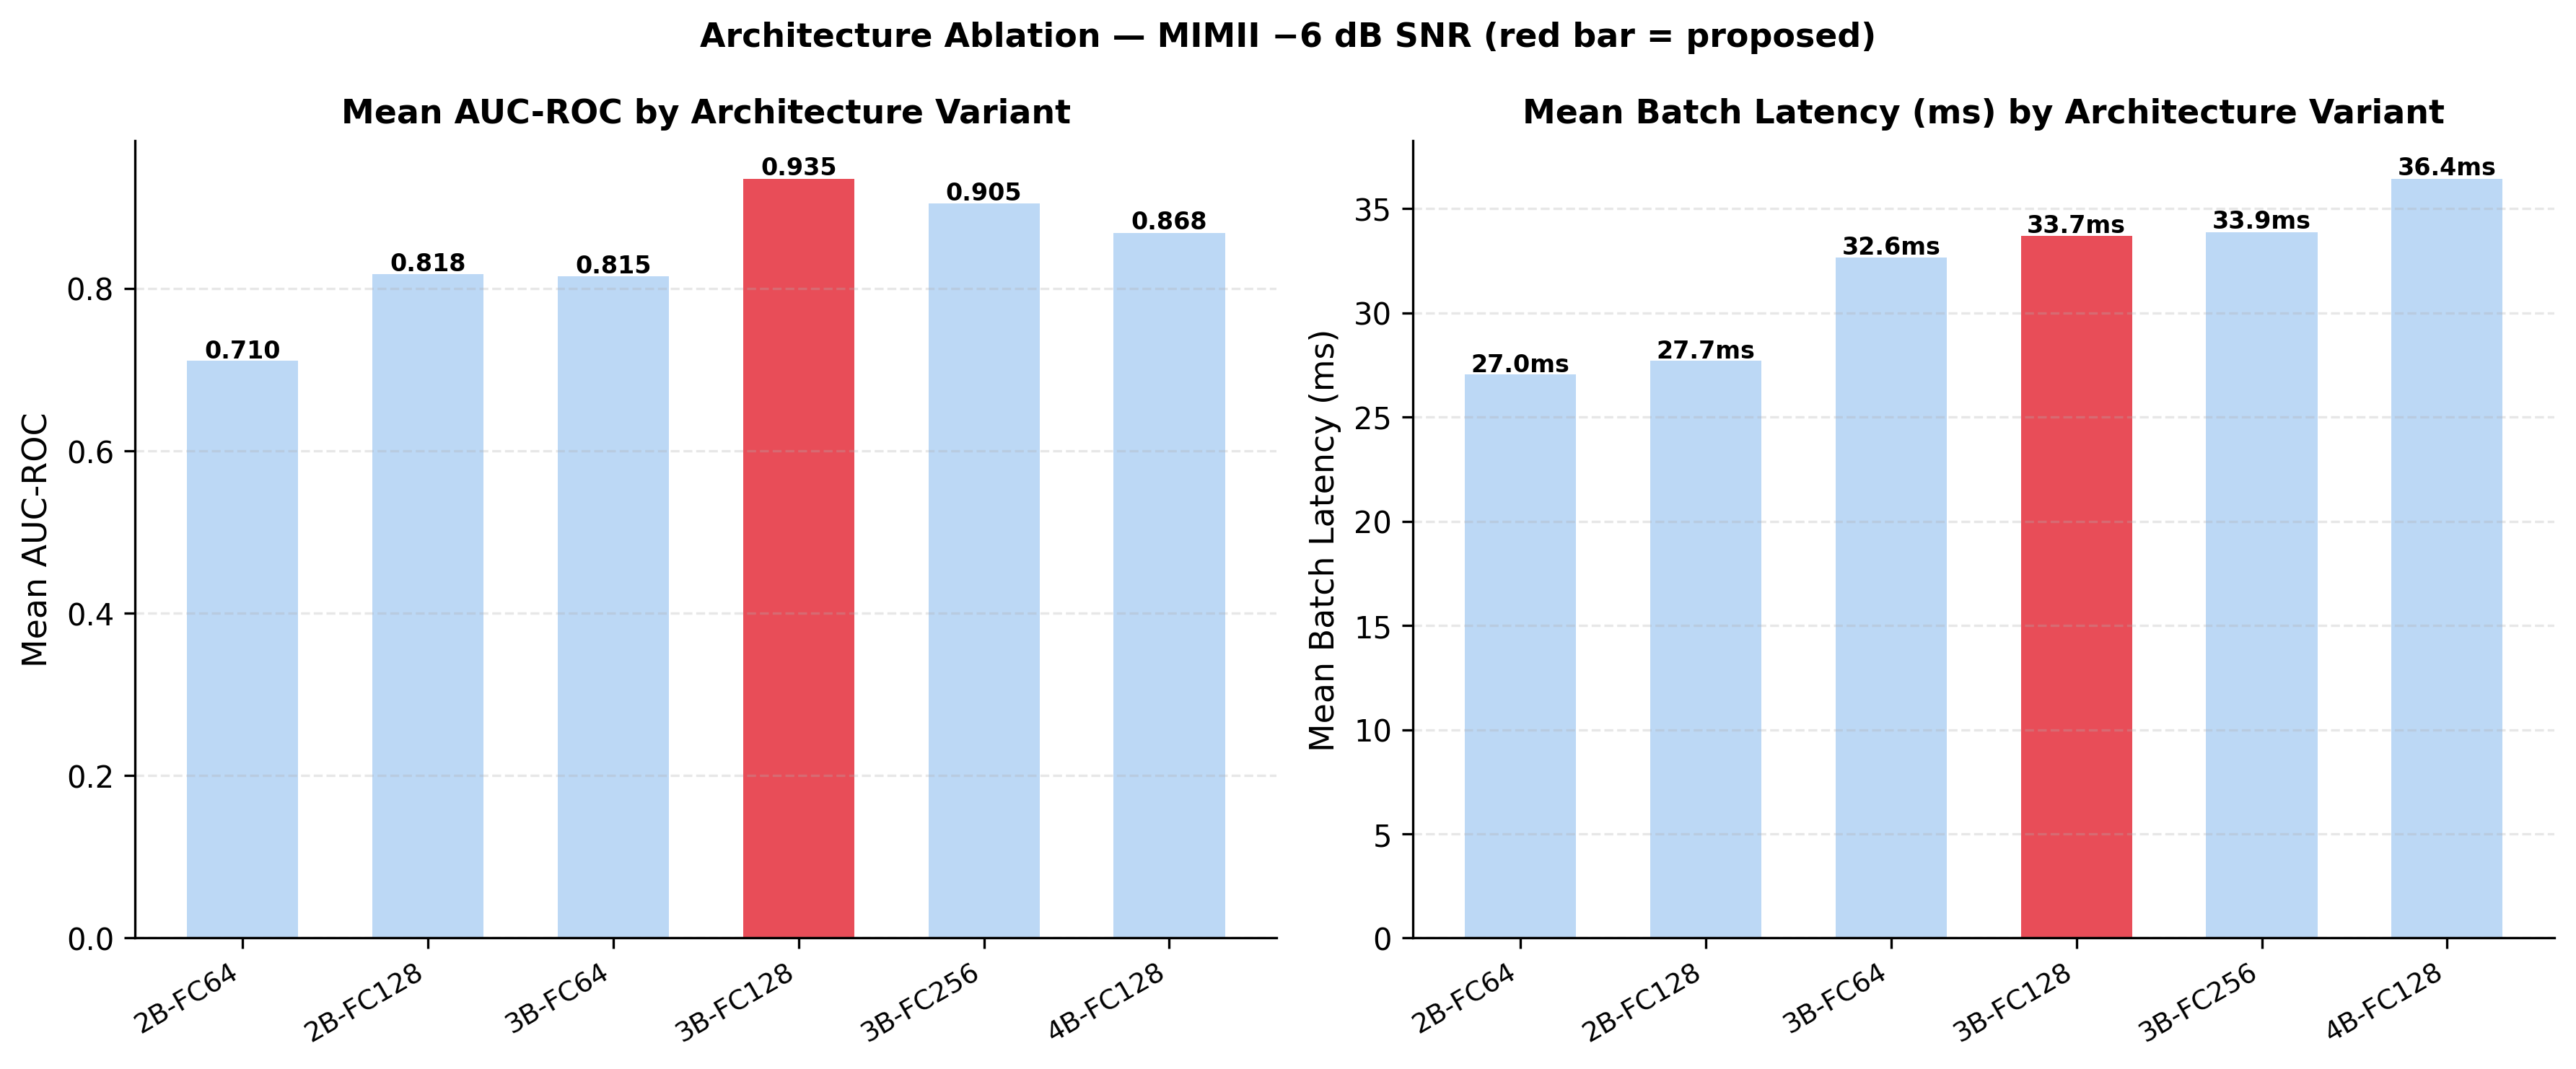
\includegraphics[width=\columnwidth]{architecture_ablation_plot.png}
\caption{Architecture ablation: mean AUC (left) and batch latency (right) per variant.}
\label{fig:arch}
\end{figure}

\subsection{SNR robustness}
\label{sec:snr}

Table~\ref{tab:snr} reports single-seed performance across the three MIMII SNR partitions (MFCC input, class-weighted loss). Fan, pump, and slider improve monotonically with SNR and exceed the 0.64 autoencoder reference at every level. The valve exhibits a non-monotonic response (0.61 at $-6$\,dB, 0.50 at $0$\,dB, 0.99 at $+6$\,dB); given the demonstrated valve seed instability, we interpret this ``SNR valley'' as a manifestation of the same unstable optimization rather than an acoustical property, and flag its spectral analysis as future work.

\begin{table}[t]
\centering
\caption{SNR sweep (MFCC input, class-weighted loss, seed 42).}
\label{tab:snr}
\begin{tabular}{llccc}
\toprule
SNR & Machine & AUC & F1 & Acc.\,(\%) \\
\midrule
$-6$\,dB & Fan & 0.9005 & 0.7289 & 83.51 \\
         & Pump & 0.9287 & 0.4235 & 76.69 \\
         & Slider & 0.9572 & 0.7781 & 90.11 \\
         & Valve & 0.6060 & 0.2443 & 59.95 \\
$0$\,dB  & Fan & 0.9881 & 0.9178 & 95.50 \\
         & Pump & 0.9592 & 0.7340 & 94.05 \\
         & Slider & 0.9917 & 0.8814 & 94.87 \\
         & Valve & 0.5000 & 0.2312 & 13.07 \\
$+6$\,dB & Fan & 0.9997 & 0.9952 & 99.73 \\
         & Pump & 0.9840 & 0.8919 & 98.10 \\
         & Slider & 0.9999 & 0.9877 & 99.51 \\
         & Valve & 0.9945 & 0.8087 & 95.80 \\
\bottomrule
\end{tabular}
\end{table}

\begin{figure}[t]
\centering
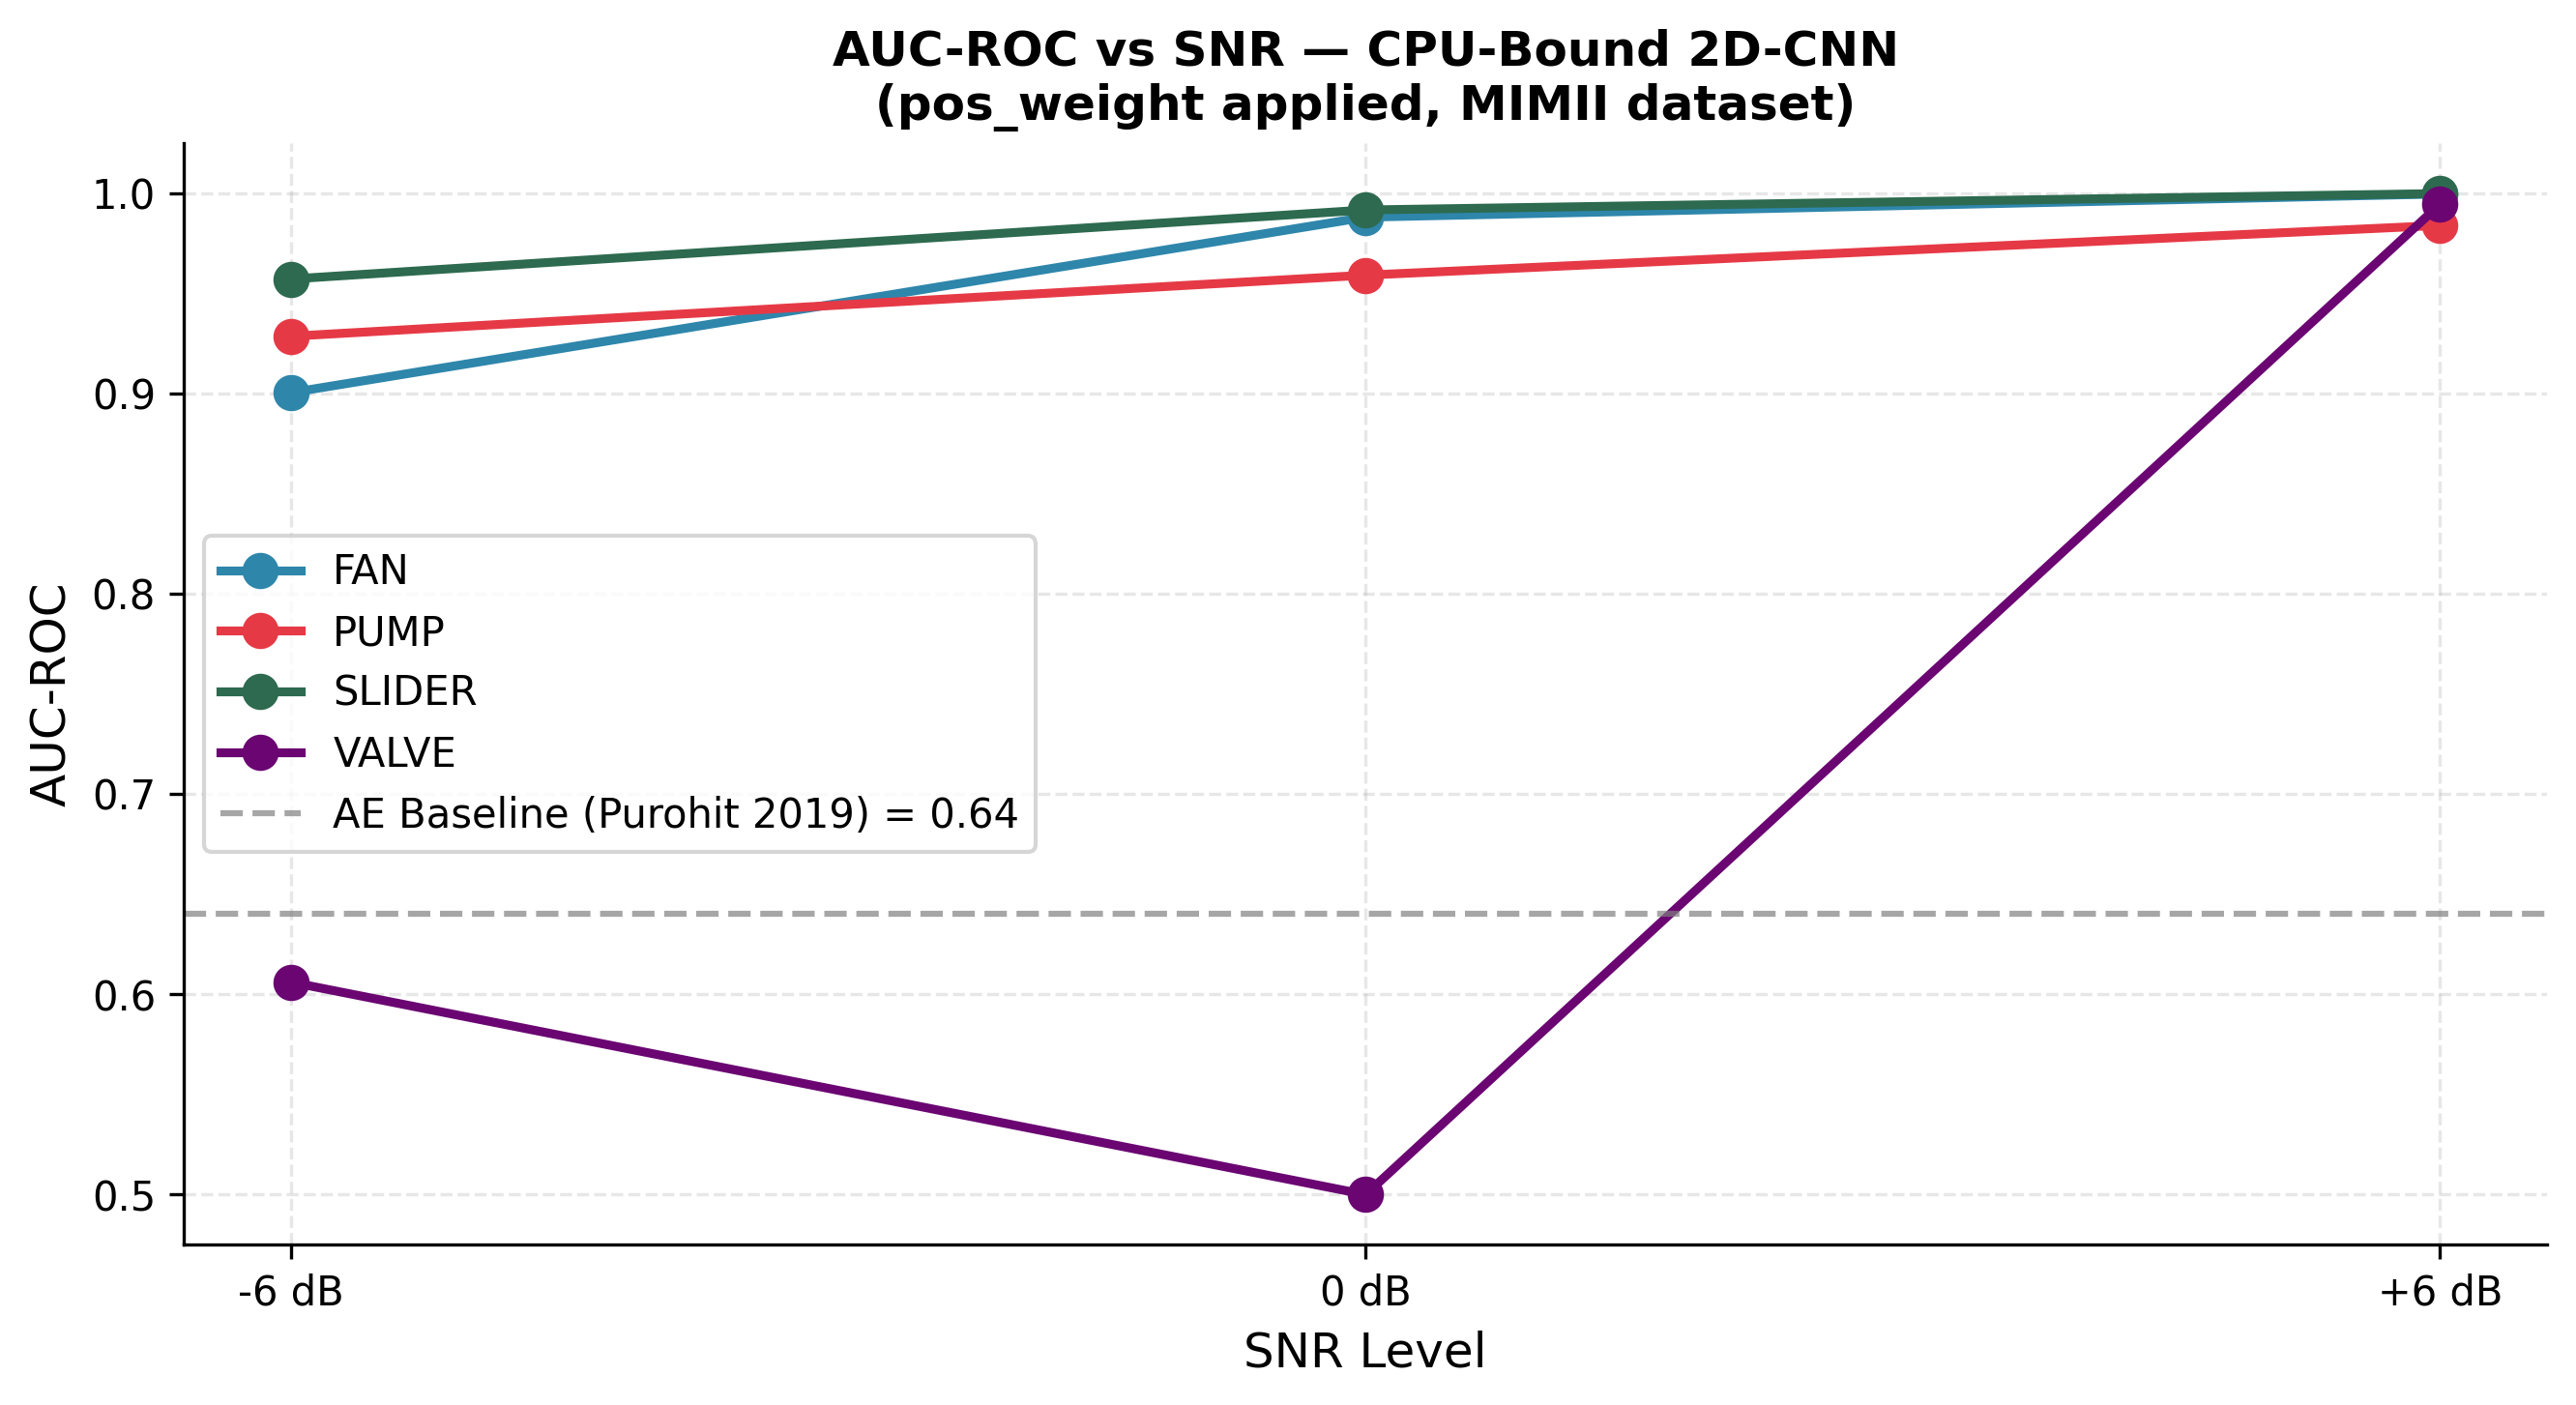
\includegraphics[width=\columnwidth]{snr_sweep_plot.png}
\caption{AUC versus SNR per machine type; dashed line: autoencoder reference ($\approx0.64$)~\cite{purohit2019mimii}.}
\label{fig:snr}
\end{figure}

\subsection{Comparison with unsupervised and supervised baselines}
\label{sec:baselines}

Table~\ref{tab:ae} situates the proposed configuration against three baselines: the published MIMII autoencoder ($\approx0.64$ mean AUC)~\cite{purohit2019mimii}, our convolutional autoencoder reproduction (``AE repr.'', Section~\ref{sec:ae-method}), and two \emph{supervised} architectures evaluated under the \emph{exact} proposed-configuration protocol---log-Mel input, class-weighted loss, the same ten seeds, 80/20 split, threshold calibration, and metrics---with only the architecture changed: the lightweight MobileNetV3~\cite{howard2019mobilenetv3} and a compact spectral--temporal fusion network in the STgram-MFN family~\cite{liu2022stgram} (``STgram-MFN-Lite''). MobileNetV3 is torchvision's \texttt{mobilenet\_v3\_small} with the first convolution replaced by a single-channel $3\times3$ stride-2 layer and the classifier head replaced by a 128-unit fully connected layer with dropout $0.2$; STgram-MFN-Lite is a compact reimplementation with two parallel three-block CNN branches (identical to the proposed model's feature extractor) applied to the log-Mel spectrogram and its first-order temporal difference, concatenated into a 128-unit embedding before the output layer. Neither baseline is pretrained; both train from random initialization under the identical ten-epoch budget of Section~\ref{sec:training}. The unsupervised reproduction confirms the published picture (mean AUC 0.616 vs.\ $\approx0.64$): reconstruction error is essentially uninformative for fan and valve at $-6$\,dB, so the value of labelled abnormal data at this noise level is large.

Three results stand out. First, the proposed 3B-FC128 attains the best mean AUC (0.959), ahead of STgram-MFN-Lite (0.942) and well ahead of MobileNetV3 (0.877); it wins fan and valve outright and trails STgram by at most 0.006 on pump and slider, so its advantage is broad rather than carried by a single machine. Second---and decisive for a deployment-oriented method---the proposed configuration combines the best mean accuracy with full seed-to-seed stability: across all forty seed-runs no seed collapses (worst per-seed AUC 0.912). MobileNetV3 is likewise free of chance-level collapse (worst seed 0.725) but at a markedly lower accuracy ceiling, whereas STgram-MFN-Lite, despite strong \emph{typical} accuracy, collapses to chance (AUC $=0.500$) on one of ten seeds for both fan and valve, inflating its per-machine standard deviation to $\pm0.13$ and $\pm0.15$. This reproduces, in a larger supervised model, the very seed-collapse pathology documented for the MFCC valve in Section~\ref{sec:multiseed}, indicating that the log-Mel + class-weighted recipe confers a robustness that added capacity alone does not. Third, the proposed model reaches this accuracy at moderate cost (Table~\ref{tab:complexity}): 3.3\,M parameters at 282 CPU frames per second---about half the size and twice the throughput of STgram-MFN-Lite (6.6\,M, 137\,FPS)---while MobileNetV3 is faster (831\,FPS) but markedly less accurate. The proposed model thus occupies the best accuracy--robustness--efficiency operating point of the three.

\begin{table}[t]
\centering
\caption{Detection performance versus unsupervised and supervised baselines at $-6$\,dB (AUC; ten-seed mean $\pm$ SD, AE values single-run). All supervised models use the identical protocol of Section~\ref{sec:protocol}; only the architecture differs. ``Worst seed'' is the minimum per-seed AUC over all machines---an index of robustness.}
\label{tab:ae}
\setlength{\tabcolsep}{3.5pt}
\begin{tabular}{lcccc}
\toprule
Machine & AE repr. & MobileNetV3 & STgram-MFN-Lite & Proposed \\
\midrule
Fan    & 0.5081 & $0.848 \pm 0.030$ & $0.886 \pm 0.129$ & $\mathbf{0.941 \pm 0.009}$ \\
Pump   & 0.6435 & $0.891 \pm 0.028$ & $\mathbf{0.950 \pm 0.010}$ & $0.945 \pm 0.011$ \\
Slider & 0.8457 & $0.959 \pm 0.010$ & $\mathbf{0.994 \pm 0.004}$ & $0.988 \pm 0.006$ \\
Valve  & 0.4661 & $0.810 \pm 0.062$ & $0.939 \pm 0.147$ & $\mathbf{0.962 \pm 0.026}$ \\
\midrule
Mean       & 0.616 & 0.877 & 0.942 & \textbf{0.959} \\
Worst seed &     & 0.725 & 0.500 & \textbf{0.912} \\
\bottomrule
\end{tabular}
\end{table}

\begin{table}[t]
\centering
\caption{Model cost under one consistent CPU benchmark (log-Mel input $1\times64\times400$, batch 16, two threads, inference only). The deployment study of Section~\ref{sec:deploy} characterizes the lighter MFCC variant of the proposed model, hence its higher absolute throughput there.}
\label{tab:complexity}
\begin{tabular}{lccc}
\toprule
Model & Params & Latency (ms) & Throughput (FPS) \\
\midrule
MobileNetV3       & 1{,}000{,}705 & 19.25  & 831.2 \\
STgram-MFN-Lite   & 6{,}600{,}897 & 117.16 & 136.6 \\
\textbf{Proposed 3B-FC128} & \textbf{3{,}300{,}577} & \textbf{56.81} & \textbf{281.6} \\
\bottomrule
\end{tabular}
\end{table}

\subsection{Generalization to unseen machine units}
\label{sec:lomo}

Table~\ref{tab:lomo} reports LOMO cross-validation under the proposed configuration (log-Mel + class-weighted loss, seed 42), now including the valve. Performance drops sharply for all four machine types---fan to near-chance ($0.521\pm0.148$), valve to $0.574\pm0.324$, pump to $0.667\pm0.106$, and slider to $0.732\pm0.223$---with large per-fold variance: individual held-out units range from 0.29 (fan id\_06) and even 0.07 (valve id\_02, an inversion in which the unit-specific signature anti-correlates with the anomaly label) up to 0.88 (slider id\_00). The supervised model evidently keys partly on unit-specific signatures. The drop closely mirrors the earlier MFCC result (fan 0.55, pump 0.69, slider 0.76), confirming that it is a property of unit-level domain shift rather than of the input representation. This delimits the method's operating envelope: it is appropriate where training data from the monitored unit are available, and unit-level domain generalization~\cite{kawaguchi2021dcase,dohi2022dcase} remains open for this model class.

\begin{table}[t]
\centering
\caption{Leave-one-machine-ID-out cross-validation under the proposed configuration (log-Mel + class-weighted loss) at $-6$\,dB (AUC; mean $\pm$ SD and 95\% bootstrap CI over four held-out identifiers).}
\label{tab:lomo}
\begin{tabular}{lcc}
\toprule
Machine & LOMO AUC & 95\% CI \\
\midrule
Fan    & $0.521 \pm 0.148$ & [0.370, 0.646] \\
Pump   & $0.667 \pm 0.106$ & [0.577, 0.775] \\
Slider & $0.732 \pm 0.223$ & [0.479, 0.879] \\
Valve  & $0.574 \pm 0.324$ & [0.269, 0.861] \\
\bottomrule
\end{tabular}
\end{table}

\subsection{Split-ratio sensitivity}
Table~\ref{tab:split} varies the train/test ratio (70/30, 80/20, 85/15; MFCC input, class-weighted loss, seed 42). Fan, pump, and slider AUCs are essentially unchanged across ratios, while the valve degrades at 85/15, where minority-class training samples become scarcest; this supports the 80/20 protocol and is consistent with the imbalance analysis above.

\begin{table}[t]
\centering
\caption{Split-ratio sensitivity (MFCC input, class-weighted loss, seed 42).}
\label{tab:split}
\begin{tabular}{lcccc}
\toprule
Split & AUC (Fan) & AUC (Pump) & AUC (Slider) & AUC (Valve) \\
\midrule
70/30 & 0.9068 & 0.9197 & 0.9600 & 0.5646 \\
\textbf{80/20} & \textbf{0.9045} & \textbf{0.9346} & \textbf{0.9610} & \textbf{0.6062} \\
85/15 & 0.8936 & 0.9424 & 0.9667 & 0.5000 \\
\bottomrule
\end{tabular}
\end{table}

% ==================================================================
\section{Deployment analysis}
\label{sec:deploy}

The deployment scenario (Fig.~\ref{fig:pipeline}) places acoustic inference exclusively on the CPU (AMD Ryzen 5 7500F, six cores) while the GPU (NVIDIA RTX 5070) is reserved for a concurrent visual workload, emulated by continuous ResNet-50~\cite{he2016resnet} inference at full load: randomly initialized weights (no pretrained checkpoint), batch size 16, $224\times224\times3$ FP32 input, back-to-back forward passes with a 20-cycle warm-up and no artificial throttling, saturating the GPU for the duration of each measurement. All benchmarks below are directly measured, under isolation and under concurrent GPU load, for the MFCC variant of the 3B-FC128 model (2.07\,M parameters) at batch size 16; the log-Mel variant was not separately benchmarked under concurrent load. Table~\ref{tab:complexity}'s isolated single-thread measurement shows the log-Mel variant is $\sim$2$\times$ costlier per inference (282 vs.\ 558\,FPS baseline throughput), and extrapolating this ratio to the measured MFCC margin below implies---but does not directly demonstrate---that the log-Mel variant would likewise clear the per-clip monitoring requirement by orders of magnitude.

\begin{figure*}[t]
\centering
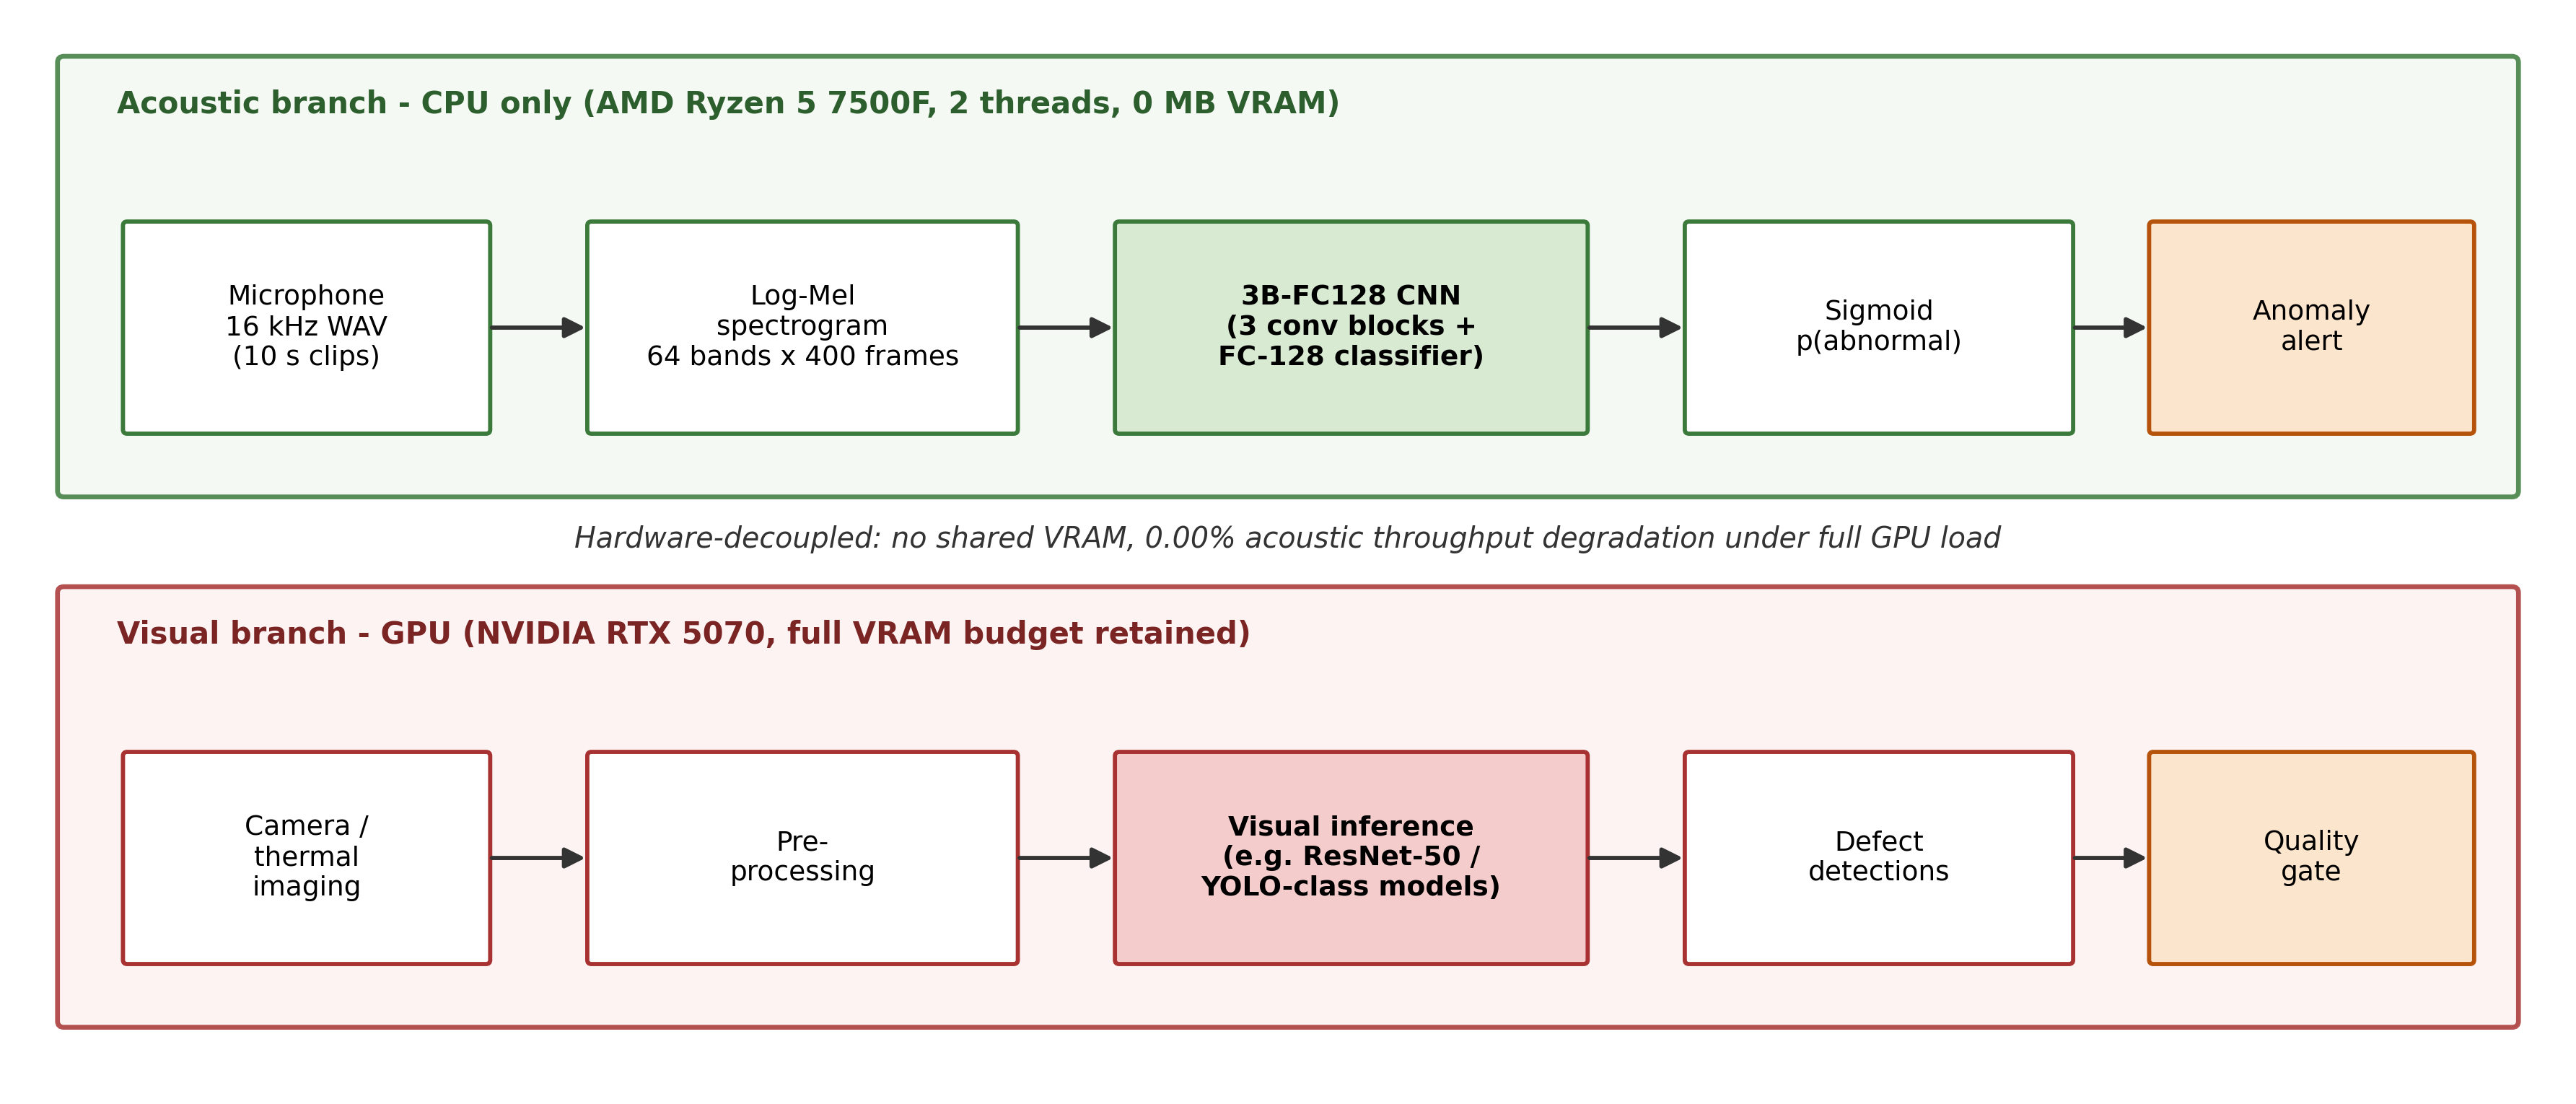
\includegraphics[width=\textwidth]{fig_pipeline.png}
\caption{Hardware-decoupled dual-stream deployment (schematic). The acoustic branch is depicted with the proposed log-Mel front end for architectural generality, but the throughput and latency numbers reported in this section were measured for the lighter MFCC variant of the same 3B-FC128 model (Section~\ref{sec:architecture}); the acoustic branch runs entirely on two CPU threads with zero VRAM use, and the visual branch retains the full GPU budget.}
\label{fig:pipeline}
\end{figure*}

\subsection{CPU versus GPU inference}
Table~\ref{tab:cpugpu} compares the two devices. The GPU is, unsurprisingly, $\sim$57$\times$ faster (31{,}654 vs.\ 558\,FPS), but the relevant question is sufficiency, not supremacy: a 10-s MIMII clip requires one inference per clip, so CPU throughput of 558\,FPS (per-sample latency 1.7--2.1\,ms) provides a real-time margin exceeding three orders of magnitude while freeing 18\,MB of VRAM and, more importantly, avoiding any GPU scheduling interaction.

\begin{table}[t]
\centering
\caption{CPU versus GPU inference (batch 16, 500 cycles).}
\label{tab:cpugpu}
\begin{tabular}{lcc}
\toprule
Metric & CPU (2 threads) & GPU (CUDA) \\
\midrule
Throughput (FPS) & 557.9 & 31{,}654.3 \\
Mean latency (ms) & 28.68 & 0.51 \\
P99 latency (ms) & 34.93 & 0.80 \\
VRAM (MB) & 0.00 & 18.01 \\
\bottomrule
\end{tabular}
\end{table}

\subsection{Thread-count sweep under GPU stress}
Table~\ref{tab:threads} and Fig.~\ref{fig:threads} report acoustic throughput in isolation and under full concurrent GPU load as a function of the PyTorch intra-op thread count. Degradation is computed as $\max(0, (\mathrm{isolated}-\mathrm{concurrent})/\mathrm{isolated}) \times 100\%$; at two threads the concurrent measurement (499.4\,FPS) nominally exceeds the isolated one (488.6\,FPS), a reversal attributable to run-to-run measurement variance rather than a genuine speedup under load, so degradation is floored at 0.0\% rather than reported as negative. Throughput scales with threads (280 FPS at one thread to 996 FPS at six), but so does interference: at six threads, concurrent degradation reaches 10.7\% as the acoustic workload competes with CUDA host-side memory operations for bandwidth, and at one thread OS scheduling interactions cost 7.4\%. The two-thread point is distinguished: across three independent measurement campaigns, two-thread degradation ranged from 0.0\% (dedicated sweep, 488.6 vs.\ 499.4 FPS) through 1.3\% (initial campaign, 569.7 vs.\ 562.2 FPS) to 6.0\% (latency-distribution campaign, 583.8 vs.\ 548.7 FPS)---always the smallest and always within single digits, while retaining roughly half a kiloframe per second of throughput. On this six-core part the heuristic $T_\mathrm{acoustic} \le N_\mathrm{cores} - T_\mathrm{GPU\,host}$ (with $\sim$4 cores absorbed by the visual pipeline's host-side work) selects the same operating point.

\begin{table}[t]
\centering
\caption{Thread sweep under concurrent GPU stress (ResNet-50 at full load).}
\label{tab:threads}
\small
\setlength{\tabcolsep}{2.5pt}
\begin{tabular}{cccccc}
\toprule
Threads & Isolated FPS & Concurrent FPS & Degr.\,(\%) & Mean (ms) & P99 (ms) \\
\midrule
1 & 280.1 & 259.4 & 7.40 & 57.1 & 68.8 \\
\textbf{2} & \textbf{488.6} & \textbf{499.4} & \textbf{0.00} & \textbf{32.8} & \textbf{37.1} \\
3 & 609.4 & 597.1 & 2.03 & 26.3 & 30.9 \\
4 & 753.7 & 738.8 & 1.96 & 21.2 & 27.1 \\
6 & 996.1 & 889.9 & 10.67 & 16.1 & 22.9 \\
\bottomrule
\end{tabular}
\end{table}

\begin{figure}[t]
\centering
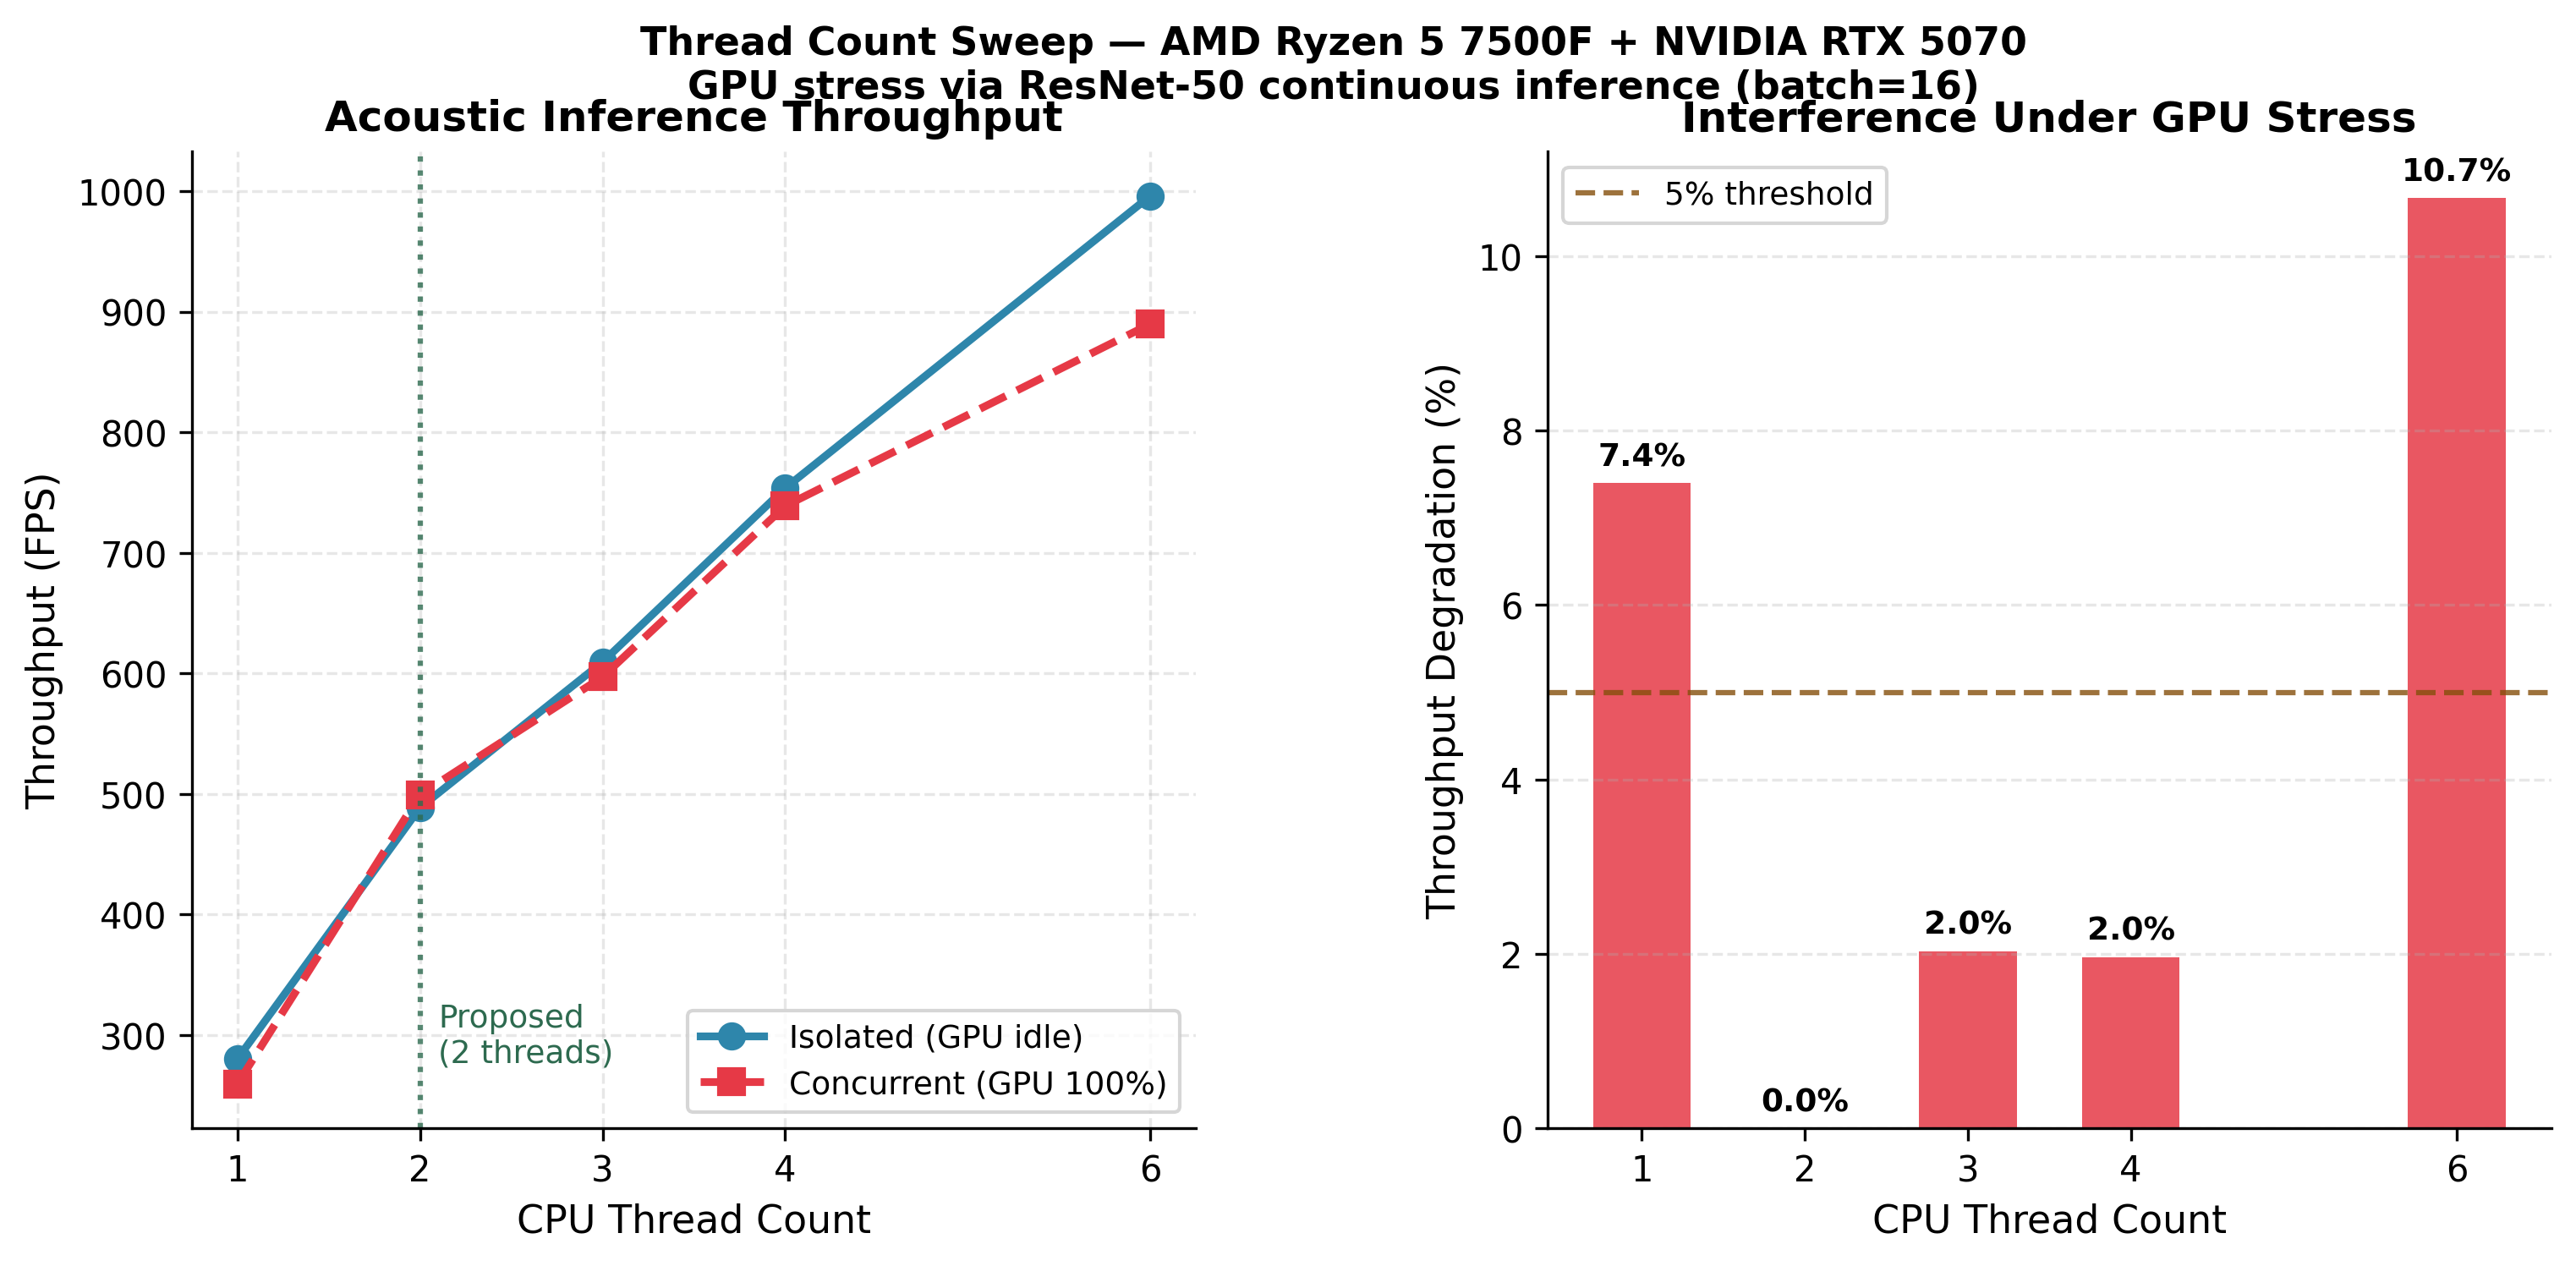
\includegraphics[width=\columnwidth]{thread_sweep_plot.png}
\caption{Thread sweep: isolated and concurrent throughput (left) and degradation under GPU stress (right).}
\label{fig:threads}
\end{figure}

\subsection{Latency distribution under concurrent load}
Figure~\ref{fig:latency} and Table~\ref{tab:latency} characterize 1{,}000 batch-inference cycles at two threads. Both conditions produce tight, unimodal distributions; the concurrent P99 batch latency of 33.5\,ms (2.09\,ms per sample) leaves a $\sim$4{,}800$\times$ real-time margin against the 10-s clip duration. The 6.4\% mean-latency increase under GPU stress reflects cache and memory-bandwidth sharing but does not threaten any plausible monitoring deadline.

\begin{table}[t]
\centering
\caption{Latency distribution at two threads (batch 16, 1{,}000 cycles).}
\label{tab:latency}
\setlength{\tabcolsep}{4pt}
\begin{tabular}{lccccc}
\toprule
Condition & Mean (ms) & P50 & P95 & P99 & FPS \\
\midrule
Isolated   & 27.41 & 27.19 & 28.88 & 31.02 & 583.8 \\
Concurrent & 29.16 & 28.96 & 31.11 & 33.45 & 548.7 \\
\bottomrule
\end{tabular}
\end{table}

\begin{figure}[t]
\centering
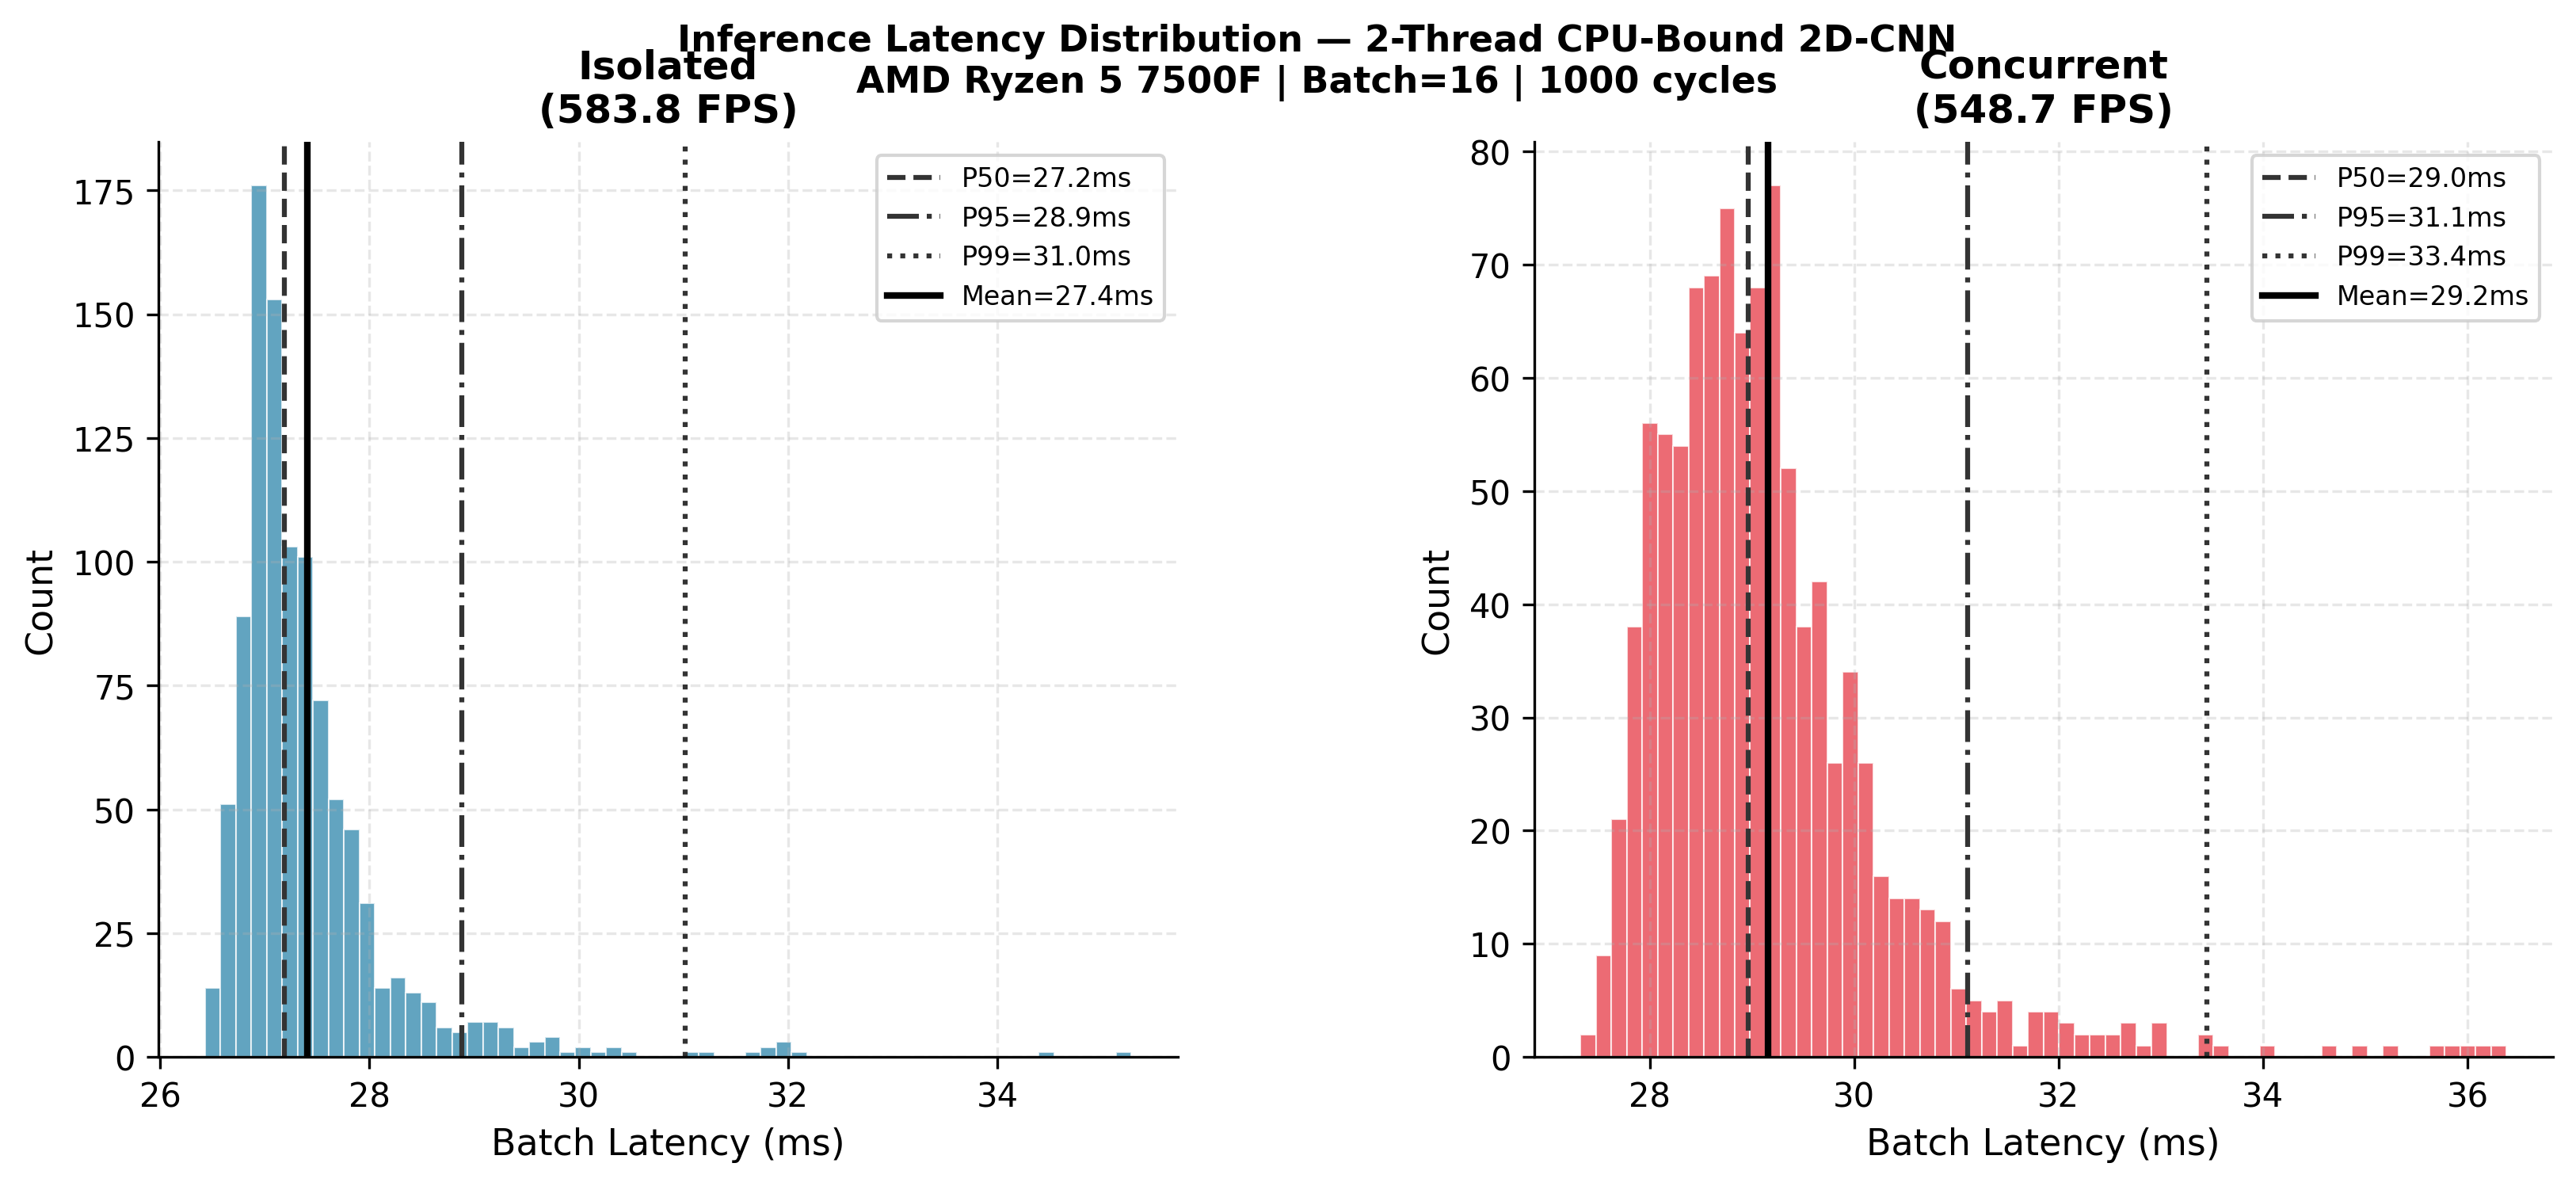
\includegraphics[width=\columnwidth]{latency_distribution_plot.png}
\caption{Batch-inference latency histograms at two threads, isolated (left) and under full GPU load (right).}
\label{fig:latency}
\end{figure}

% ==================================================================
\section{Discussion}
\label{sec:discussion}

\paragraph{What enables minority-class detection under severe noise} The collapse analysis localizes the failure to an interaction of loss prior and representation. Re-weighting rebalances the gradient but cannot conjure discriminative structure that the input has destroyed: MFCC's cepstral compaction removes the inter-band co-occurrence patterns of broadband valve transients, so the re-weighted optimizer has no consistent minority-class signal to fit and falls into seed-dependent solutions---recovering occasionally (which explains optimistic single-run numbers in the literature and in our own ablation table) and collapsing more often. Log-Mel input restores that structure, and only the joint intervention yields reliable recovery. The practical prescription for imbalanced industrial ASD is therefore: retain full spectral energy maps, re-weight the loss, and \emph{always} validate over multiple seeds before trusting minority-class metrics.

\paragraph{Capacity is not monotonic under imbalance} Both a wider classifier (FC-256) and a deeper extractor (4B) degraded the most imbalanced category while leaving balanced categories intact---a useful caution against reflexive scaling when minority-class generalization is the binding constraint. The same lesson recurs in the baseline comparison (Section~\ref{sec:baselines}): the 6.6\,M-parameter STgram-MFN-Lite, though strong on average, collapses on individual seeds where the 3.3\,M proposed model never does---added capacity is no substitute for the representation--loss recipe that underwrites stability.

\paragraph{Deployment} The interference measurements support a simple architectural rule for shared edge nodes: pin the acoustic model to a small number of CPU threads (here two of six), leave the GPU and the remaining cores to the visual pipeline, and the two streams coexist with single-digit interference and zero memory contention. The absolute throughput ($\approx$500\,FPS of 10-s clips) is so far above the monitoring requirement that the CPU's 57$\times$ throughput disadvantage versus the GPU is operationally irrelevant.

\paragraph{Scope} The LOMO results are a deliberate transparency exercise: supervised in-domain excellence (mean AUC 0.94--0.99) coexists with weak unit-level transfer (mean AUC 0.52--0.73, with individual folds spanning chance to 0.88). Claims of deployability therefore extend to monitored units represented in training data; cross-unit deployment requires domain generalization techniques that are outside this paper's scope.

% ==================================================================
\section{Limitations}
\label{sec:limitations}

(i)~All detection results derive from MIMII; transfer to other acoustic environments, microphone arrays, and machine classes is untested. (ii)~The supervised protocol requires labelled abnormal recordings, which many plants lack at commissioning time; the unsupervised DCASE protocol addresses a complementary scenario, and the comparison in Table~\ref{tab:ae} should be read accordingly. (iii)~Valve training remains seed-sensitive even in the proposed configuration to the extent quantified in Table~\ref{tab:multiseed}; per-seed distributions are reported precisely so that downstream users can judge this risk. (iv)~Deployment numbers are specific to one CPU/GPU platform; ARM-class edge processors require separate characterization. (v)~The SNR-valley behaviour of the valve at 0\,dB is observed but not mechanistically explained. (vi)~The representation study compares only cepstral (MFCC) and filterbank (log-Mel) inputs; psychoacoustic and learnable time--frequency front-ends~\cite{wissbrock2024more} are promising alternatives not evaluated here. (vii)~The supervised baselines (MobileNetV3, STgram-MFN-Lite) are compact reimplementations evaluated under our common ten-epoch protocol for an equal-footing comparison; the per-seed collapse observed for the fusion baseline is a property of that shared training budget, not necessarily of the original STgram-MFN with its own tuned regime.

% ==================================================================
\section{Conclusions}
\label{sec:conclusion}

This study characterized a lightweight 2D-CNN for supervised acoustic anomaly detection on MIMII at $-6$\,dB SNR, with three principal findings. First, with log-Mel input and class-weighted loss, the 3B-FC128 model achieves ten-seed mean AUCs of \msFanAuc{} (fan), \msPumpAuc{} (pump), \msSliderAuc{} (slider), and \msValveAuc{} (valve), far exceeding reconstruction-based baselines at this noise level and, under one identical protocol, attaining the best mean AUC of the three supervised architectures compared while never collapsing on any seed---unlike the STgram-MFN fusion model---and at half its parameter count. Second, the severe-imbalance valve category exhibits decision collapse whose repair requires the joint application of full-spectrum log-Mel features and loss re-weighting, and whose single-run metrics are seed-unstable---a methodological caution for the field. Third, the MFCC variant of the model sustains roughly half a kiloframe per second of CPU-only inference on two threads of a commodity six-core processor with zero VRAM use and at most single-digit throughput degradation under full concurrent GPU load; the costlier log-Mel variant still clears the real-time requirement by orders of magnitude. Together these results validate hardware-decoupled multimodal deployment at the industrial edge for machine units represented in training data. To support reproducibility, the code, trained weights, and per-seed logs are available at an anonymized repository (Data availability statement) and will be deposited under the authors' identities in a public repository upon acceptance.

% ==================================================================
\section*{CRediT authorship contribution statement}
\textbf{Mohammad Raziul Hasan Rifat Sakar:} Conceptualization, Methodology, Software, Investigation, Writing -- original draft. \textbf{Labani Akter:} Validation, Data curation, Visualization, Writing -- review \& editing. \textbf{Tao Zhang:} Supervision, Resources, Project administration, Writing -- review \& editing. \textbf{Saleh Mahamat Aboubakar OUSMANE:} Validation. \textbf{Boudjelkha Mohammed Djamel EDDINE:} Writing -- review \& editing.

\section*{Declaration of competing interest}
The authors declare that they have no known competing financial interests or personal relationships that could have appeared to influence the work reported in this paper.

\section*{Funding}
This paper is supported by 2025 Huai'an City Basic Research Program (Joint Special Project, HABL202501).

\section*{Data availability}
The MIMII dataset is publicly available~\cite{purohit2019mimii}. To support reproducibility, the experiment code, per-seed logs, and trained model weights are available at an anonymized repository, \url{https://anonymous.4open.science/r/Acoustic-Anomaly-Detection-FB56/}, and will be deposited under the authors' identities in a public repository upon acceptance.

\section*{Declaration of generative AI and AI-assisted technologies in the manuscript preparation process}
During the preparation of this work the author(s) used Claude (Anthropic) in order to assist with editing and formatting of the manuscript text. After using this tool, the author(s) reviewed and edited the content as needed and take full responsibility for the content of the published article.

\bibliographystyle{elsarticle-num}
\bibliography{references}

\end{document}
